\section{Results and Discussion}
\label{sec:results}

\begin{figure*}[t]
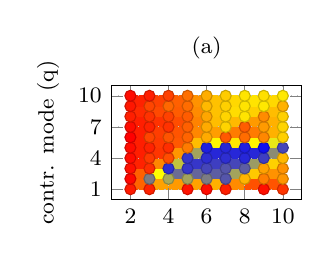
\begin{tikzpicture}
\begin{axis}
[
width=0.33\textwidth,
height=0.25\textwidth,
style={font=\footnotesize},
grid=major,
grid style={dotted},
align=center,
%xlabel={tensor order},
ylabel={contr. mode (q)},
title={{(a)}}, %  bgemm, asymmetric
scaled ticks=false,
zlabel={GFlops},
view={0}{90}, 
ytick={1,4,7,10},
xtick={2,4,6,8,10},
xmin=1, xmax=11,
ymin=0, ymax=11,
try min ticks=8,
zmin=300, zmax=2300,
point meta min=300, point meta max=2300,
colormap/hot, 
samples=50,
%colorbar sampled,
%colorbar/width=0.2cm,
%colorbar style={
%	point meta min=300, point meta max=2300,
%	samples=50,
%	font=\footnotesize,
%	ytick={300,1300,2300},
%	yticklabels={0.3,1.3,2.3},
%	%title={\scriptsize Gflops},
%	%ylabel={\scriptsize Gflops},
%}
]
%\addplot3[mesh, scatter,samples=50,shader=interp]
%\addplot3[only marks, mesh, scatter,scatter src=z,samples=50,] % z buffer=sort, scatter src=z,
\addplot3[contour filled={number=100},scatter,shader=flat,samples=50]
%\addplot3+[mesh,scatter,shader=flat corner,samples=50, only marks, mark size=2]
coordinates{
	
(2.000,1.000,2142.734) (2.000,2.000,2241.014) (2.000,3.000,2205.546) (2.000,4.000,2226.263) (2.000,5.000,2232.877) (2.000,6.000,2281.816) (2.000,7.000,2222.317) (2.000,8.000,2122.831) (2.000,9.000,2166.437) (2.000,10.000,2231.354) 

(3.000,1.000,2104.803) (3.000,2.000,620.292) (3.000,3.000,2053.810) (3.000,4.000,1989.460) (3.000,5.000,2100.108) (3.000,6.000,1923.866) (3.000,7.000,2109.798) (3.000,8.000,2032.918) (3.000,9.000,1931.835) (3.000,10.000,2137.550) 

(4.000,1.000,2303.560) (4.000,2.000,742.055) (4.000,3.000,436.752) (4.000,4.000,1889.266) (4.000,5.000,2050.848) (4.000,6.000,1845.429) (4.000,7.000,2029.757) (4.000,8.000,1947.246) (4.000,9.000,1753.968) (4.000,10.000,1945.836) 

(5.000,1.000,2197.949) (5.000,2.000,727.736) (5.000,3.000,441.734) (5.000,4.000,458.055) (5.000,5.000,1643.657) (5.000,6.000,1763.676) (5.000,7.000,1793.195) (5.000,8.000,1799.906) (5.000,9.000,1726.622) (5.000,10.000,1710.693) 

(6.000,1.000,2225.857) (6.000,2.000,621.489) (6.000,3.000,489.438) (6.000,4.000,435.500) (6.000,5.000,386.554) (6.000,6.000,1410.907) (6.000,7.000,1419.437) (6.000,8.000,1428.795) (6.000,9.000,1330.280) (6.000,10.000,1386.923) 

(7.000,1.000,2137.668) (7.000,2.000,530.662) (7.000,3.000,532.587) (7.000,4.000,439.307) (7.000,5.000,400.923) (7.000,6.000,1835.402) (7.000,7.000,1186.143) (7.000,8.000,1195.514) (7.000,9.000,1211.432) (7.000,10.000,1230.143) 

(8.000,1.000,2411.000) (8.000,2.000,1340.829) (8.000,3.000,546.729) (8.000,4.000,405.255) (8.000,5.000,381.061) (8.000,6.000,1724.053) (8.000,7.000,1816.684) (8.000,8.000,1103.276) (8.000,9.000,1109.365) (8.000,10.000,1119.582) 

(9.000,1.000,2215.896) (9.000,2.000,1637.409) (9.000,3.000,1448.314) (9.000,4.000,477.752) (9.000,5.000,353.959) (9.000,6.000,1596.361) (9.000,7.000,1496.308) (9.000,8.000,1566.431) (9.000,9.000,1085.107) (9.000,10.000,1135.908) 

(10.000,1.000,2011.147) (10.000,2.000,1504.412) (10.000,3.000,1538.421) (10.000,4.000,1335.732) (10.000,5.000,483.993) (10.000,6.000,1202.734) (10.000,7.000,1197.316) (10.000,8.000,1213.834) (10.000,9.000,1362.208) (10.000,10.000,1087.708)


};
\end{axis}
\end{tikzpicture}
\hfill
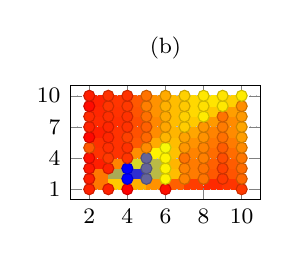
\begin{tikzpicture}
\begin{axis}
[
width=0.33\textwidth,
height=0.25\textwidth,
style={font=\footnotesize},
grid=major,
grid style={dotted},
align=center,
%xlabel={tensor order},
%ylabel={contr. mode (q)},
title={{(b)}}, %  ompfor<2d-slice> ttm<par-loops,seq-blas,$q$-slice>, asymmetric
scaled ticks=false,
zlabel={GFlops},
view={0}{90}, 
%view={-45}{45}, 
ytick={1,4,7,10},
xtick={2,4,6,8,10},
xmin=1, xmax=11,
ymin=0, ymax=11,
try min ticks=8,
zmin=300, zmax=2300,
point meta min=300, point meta max=2300,
colormap/hot, 
samples=50,
%colorbar sampled,
%colorbar/width=0.2cm,
%colorbar style={
%	point meta min=300, point meta max=2300,
%	samples=50,
%	font=\footnotesize,
%	ytick={300,1300,2300},
%	yticklabels={0.3,1.3,2.3},
%	%title={\scriptsize Gflops},
%	%ylabel={\scriptsize Gflops},
%}
]
%\addplot3[mesh, scatter,samples=50,shader=interp]
%\addplot3[only marks, mesh, scatter,scatter src=z,samples=50,] % z buffer=sort, scatter src=z,
\addplot3[contour filled={number=100},scatter,shader=flat,samples=50]
%\addplot3+[mesh,scatter,shader=flat corner,samples=50, only marks, mark size=2]
coordinates{

(2.000,1.000,2107.002) (2.000,2.000,2127.162) (2.000,3.000,2176.298) (2.000,4.000,2215.649) (2.000,5.000,1837.632) (2.000,6.000,2241.609) (2.000,7.000,2101.558) (2.000,8.000,2075.436) (2.000,9.000,2236.130) (2.000,10.000,2133.353) 

(3.000,1.000,2119.523) (3.000,2.000,167.437) (3.000,3.000,2112.420) (3.000,4.000,1989.285) (3.000,5.000,2041.921) (3.000,6.000,2084.201) (3.000,7.000,2080.454) (3.000,8.000,2046.614) (3.000,9.000,2013.009) (3.000,10.000,2024.421) 

(4.000,1.000,2285.299) (4.000,2.000,314.287) (4.000,3.000,311.849) (4.000,4.000,2011.869) (4.000,5.000,2039.029) (4.000,6.000,1944.642) (4.000,7.000,2023.178) (4.000,8.000,2033.385) (4.000,9.000,1992.379) (4.000,10.000,2039.303) 

(5.000,1.000,2475.804) (5.000,2.000,568.291) (5.000,3.000,562.230) (5.000,4.000,562.587) (5.000,5.000,1564.667) (5.000,6.000,1756.890) (5.000,7.000,1791.524) (5.000,8.000,1712.024) (5.000,9.000,1626.887) (5.000,10.000,1695.764) 

(6.000,1.000,2218.038) (6.000,2.000,1025.980) (6.000,3.000,1034.039) (6.000,4.000,1026.350) (6.000,5.000,945.367) (6.000,6.000,1340.191) (6.000,7.000,1422.937) (6.000,8.000,1402.244) (6.000,9.000,1375.707) (6.000,10.000,1411.432) 

(7.000,1.000,2307.246) (7.000,2.000,1602.074) (7.000,3.000,1617.348) (7.000,4.000,1682.539) (7.000,5.000,1516.443) (7.000,6.000,1446.511) (7.000,7.000,1229.353) (7.000,8.000,1202.606) (7.000,9.000,1245.855) (7.000,10.000,1211.880) 

(8.000,1.000,2441.539) (8.000,2.000,1699.771) (8.000,3.000,1686.405) (8.000,4.000,1622.372) (8.000,5.000,1600.438) (8.000,6.000,1530.707) (8.000,7.000,1508.466) (8.000,8.000,1073.808) (8.000,9.000,1123.363) (8.000,10.000,1096.486) 

(9.000,1.000,2330.060) (9.000,2.000,1985.056) (9.000,3.000,1941.312) (9.000,4.000,1892.533) (9.000,5.000,1805.699) (9.000,6.000,1706.515) (9.000,7.000,1658.818) (9.000,8.000,1693.350) (9.000,9.000,1093.684) (9.000,10.000,1112.530) 

(10.000,1.000,1988.818) (10.000,2.000,1750.516) (10.000,3.000,1728.226) (10.000,4.000,1678.568) (10.000,5.000,1576.395) (10.000,6.000,1476.492) (10.000,7.000,1429.733) (10.000,8.000,1496.574) (10.000,9.000,1557.162) (10.000,10.000,1068.719) 


};
\end{axis}
\end{tikzpicture}
\hfill
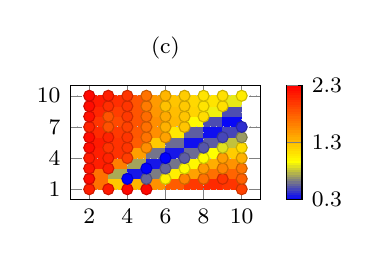
\begin{tikzpicture}
\begin{axis}
[
width=0.33\textwidth,
height=0.25\textwidth,
style={font=\footnotesize},
grid=major,
grid style={dotted},
align=center,
%xlabel={tensor order},
%ylabel={contr. mode (q)},
title={{(c)}}, %  ompfor<qd-slice> ttm<par-loops,seq-blas,$q$-slice>, asymmetric
scaled ticks=false,
zlabel={GFlops},
view={0}{90}, 
%view={-45}{45}, 
ytick={1,4,7,10},
xtick={2,4,6,8,10},
%xmin=2, xmax=10,
%ymin=1, ymax=10,
xmin=1, xmax=11,
ymin=0, ymax=11,
try min ticks=8,
zmin=300, zmax=2300,
point meta min=300, point meta max=2300,
%colormap/jet, 
colormap/hot, 
%colormap/blackwhite,
%colormap={whiteblack}{indices of colormap={\pgfplotscolormaplastindexof{blackwhite},...,0 of blackwhite}},
samples=50,
%colormap access=piecewise const,
colorbar sampled,
colorbar/width=0.2cm,
colorbar style={
	point meta min=300, point meta max=2300,
	samples=50,
	font=\footnotesize,
	ytick={300,1300,2300},
	yticklabels={0.3,1.3,2.3},
	%title={\scriptsize Gflops},
	%ylabel={\scriptsize Gflops},
}
]
%\addplot3[mesh, scatter,samples=50,shader=interp]
%\addplot3[only marks, mesh, scatter,scatter src=z,samples=50,] % z buffer=sort, scatter src=z,
\addplot3[contour filled={number=100},scatter,shader=flat,samples=50]
%\addplot3+[mesh,scatter,shader=flat corner,samples=50, only marks, mark size=2]
coordinates{

(2.000,1.000,2134.021) (2.000,2.000,2224.864) (2.000,3.000,2184.477) (2.000,4.000,2142.541) (2.000,5.000,2229.439) (2.000,6.000,2238.772) (2.000,7.000,2105.091) (2.000,8.000,2201.214) (2.000,9.000,2232.448) (2.000,10.000,2240.926) 

(3.000,1.000,2146.896) (3.000,2.000,167.544) (3.000,3.000,2121.476) (3.000,4.000,2105.304) (3.000,5.000,2027.717) (3.000,6.000,2104.722) (3.000,7.000,1866.561) (3.000,8.000,1855.180) (3.000,9.000,2041.894) (3.000,10.000,2122.692) 

(4.000,1.000,2244.985) (4.000,2.000,313.766) (4.000,3.000,167.879) (4.000,4.000,1973.457) (4.000,5.000,2013.391) (4.000,6.000,2010.678) (4.000,7.000,1949.136) (4.000,8.000,1989.844) (4.000,9.000,2017.192) (4.000,10.000,2015.899) 

(5.000,1.000,2250.694) (5.000,2.000,574.277) (5.000,3.000,315.908) (5.000,4.000,166.343) (5.000,5.000,1559.782) (5.000,6.000,1688.138) (5.000,7.000,1711.412) (5.000,8.000,1721.389) (5.000,9.000,1653.587) (5.000,10.000,1691.902) 

(6.000,1.000,2403.465) (6.000,2.000,1026.371) (6.000,3.000,576.699) (6.000,4.000,312.020) (6.000,5.000,160.917) (6.000,6.000,1443.174) (6.000,7.000,1370.699) (6.000,8.000,1414.204) (6.000,9.000,1283.900) (6.000,10.000,1351.446) 

(7.000,1.000,2305.894) (7.000,2.000,1613.830) (7.000,3.000,988.435) (7.000,4.000,554.792) (7.000,5.000,290.305) (7.000,6.000,157.356) (7.000,7.000,1270.432) (7.000,8.000,1266.914) (7.000,9.000,1255.620) (7.000,10.000,1224.914) 

(8.000,1.000,2437.239) (8.000,2.000,1706.219) (8.000,3.000,1489.110) (8.000,4.000,999.755) (8.000,5.000,531.137) (8.000,6.000,280.182) (8.000,7.000,148.892) (8.000,8.000,1156.621) (8.000,9.000,1110.478) (8.000,10.000,1116.944) 

(9.000,1.000,2355.395) (9.000,2.000,2003.839) (9.000,3.000,1603.752) (9.000,4.000,1477.309) (9.000,5.000,887.839) (9.000,6.000,492.554) (9.000,7.000,262.294) (9.000,8.000,150.408) (9.000,9.000,1129.997) (9.000,10.000,1121.143) 

(10.000,1.000,1944.959) (10.000,2.000,1789.054) (10.000,3.000,1665.441) (10.000,4.000,1375.291) (10.000,5.000,1147.731) (10.000,6.000,715.205) (10.000,7.000,422.658) (10.000,8.000,236.076) (10.000,9.000,136.520) (10.000,10.000,1078.495) 


};
\end{axis}
\end{tikzpicture}


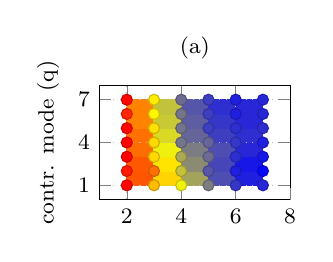
\begin{tikzpicture}
\begin{axis}
[
width=0.33\textwidth,
height=0.25\textwidth,
style={font=\footnotesize},
grid=major,
grid style={dotted},
align=center,
%xlabel={tensor order},
ylabel={contr. mode (q)},
title={{(a)}}, %  bgemm, asymmetric
scaled ticks=false,
zlabel={GFlops},
view={0}{90}, 
ytick={1,4,7,10},
xtick={2,4,6,8},
xmin=1, xmax=8,
ymin=0, ymax=8,
try min ticks=8,
zmin=0, zmax=2600,
point meta min=0, point meta max=2600,
colormap/hot, 
samples=50,
%colorbar sampled,
%colorbar/width=0.2cm,
%colorbar style={
%	point meta min=300, point meta max=2300,
%	samples=50,
%	font=\footnotesize,
%	ytick={300,1300,2300},
%	yticklabels={0.3,1.3,2.3},
%	%title={\scriptsize Gflops},
%	%ylabel={\scriptsize Gflops},
%}
]
%\addplot3[mesh, scatter,samples=50,shader=interp]
%\addplot3[only marks, mesh, scatter,scatter src=z,samples=50,] % z buffer=sort, scatter src=z,
\addplot3[contour filled={number=100},scatter,shader=flat,samples=50]
%\addplot3+[mesh,scatter,shader=flat corner,samples=50, only marks, mark size=2]
coordinates{

(2.000,1.000,2527.923) (2.000,2.000,2398.051) (2.000,3.000,2573.521) (2.000,4.000,2570.296) (2.000,5.000,2540.651) (2.000,6.000,2326.903) (2.000,7.000,2545.629) 

(3.000,1.000,1312.517) (3.000,2.000,1835.211) (3.000,3.000,1133.124) (3.000,4.000,1120.384) (3.000,5.000,1066.704) (3.000,6.000,915.932) (3.000,7.000,997.168) 

(4.000,1.000,825.045) (4.000,2.000,655.270) (4.000,3.000,579.750) (4.000,4.000,390.794) (4.000,5.000,411.134) (4.000,6.000,409.619) (4.000,7.000,375.457) 

(5.000,1.000,420.343) (5.000,2.000,308.678) (5.000,3.000,377.118) (5.000,4.000,348.232) (5.000,5.000,216.877) (5.000,6.000,232.073) (5.000,7.000,218.457) 

(6.000,1.000,206.774) (6.000,2.000,119.299) (6.000,3.000,167.691) (6.000,4.000,183.571) (6.000,5.000,179.989) (6.000,6.000,126.876) (6.000,7.000,128.135) 

(7.000,1.000,150.823) (7.000,2.000,33.170) (7.000,3.000,83.979) (7.000,4.000,128.221) (7.000,5.000,157.368) (7.000,6.000,143.557) (7.000,7.000,133.647) 


};
\end{axis}
\end{tikzpicture}
\hfill
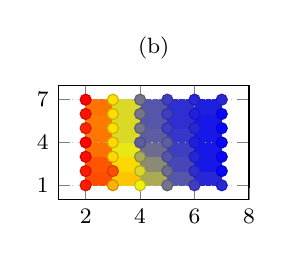
\begin{tikzpicture}
\begin{axis}
[
width=0.33\textwidth,
height=0.25\textwidth,
style={font=\footnotesize},
grid=major,
grid style={dotted},
align=center,
%xlabel={tensor order},
%ylabel={contr. mode (q)},
title={{(b)}}, %  ompfor<2d-slice> ttm<par-loops,seq-blas,$q$-slice>, asymmetric
scaled ticks=false,
zlabel={GFlops},
view={0}{90}, 
%view={-45}{45}, 
ytick={1,4,7,10},
xtick={2,4,6,8},
xmin=1, xmax=8,
ymin=0, ymax=8,
try min ticks=8,
zmin=0, zmax=2600,
point meta min=0, point meta max=2600,
colormap/hot, 
samples=50,
%colorbar sampled,
%colorbar/width=0.2cm,
%colorbar style={
%	point meta min=300, point meta max=2300,
%	samples=50,
%	font=\footnotesize,
%	ytick={300,1300,2300},
%	yticklabels={0.3,1.3,2.3},
%	%title={\scriptsize Gflops},
%	%ylabel={\scriptsize Gflops},
%}
]
%\addplot3[mesh, scatter,samples=50,shader=interp]
%\addplot3[only marks, mesh, scatter,scatter src=z,samples=50,] % z buffer=sort, scatter src=z,
\addplot3[contour filled={number=100},scatter,shader=flat,samples=50]
%\addplot3+[mesh,scatter,shader=flat corner,samples=50, only marks, mark size=2]
coordinates{

(2.000,1.000,2394.429) (2.000,2.000,2411.386) (2.000,3.000,2508.441) (2.000,4.000,2549.390) (2.000,5.000,2334.831) (2.000,6.000,2454.725) (2.000,7.000,2556.685) 

(3.000,1.000,1395.054) (3.000,2.000,2055.946) (3.000,3.000,1121.102) (3.000,4.000,1120.659) (3.000,5.000,1089.377) (3.000,6.000,1102.959) (3.000,7.000,1078.957) 

(4.000,1.000,819.991) (4.000,2.000,729.342) (4.000,3.000,579.869) (4.000,4.000,334.133) (4.000,5.000,390.153) (4.000,6.000,407.045) (4.000,7.000,394.057) 

(5.000,1.000,414.803) (5.000,2.000,369.532) (5.000,3.000,295.077) (5.000,4.000,318.473) (5.000,5.000,209.139) (5.000,6.000,214.825) (5.000,7.000,223.888) 

(6.000,1.000,208.097) (6.000,2.000,156.950) (6.000,3.000,141.868) (6.000,4.000,119.992) (6.000,5.000,134.757) (6.000,6.000,126.271) (6.000,7.000,133.034) 

(7.000,1.000,151.228) (7.000,2.000,27.225) (7.000,3.000,30.634) (7.000,4.000,31.221) (7.000,5.000,30.322) (7.000,6.000,31.152) (7.000,7.000,133.496) 


};
\end{axis}
\end{tikzpicture}
\hfill
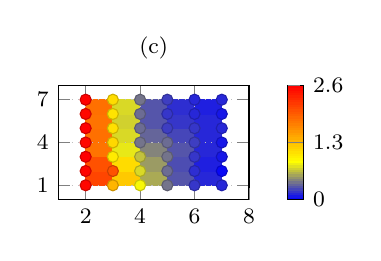
\begin{tikzpicture}
\begin{axis}
[
width=0.33\textwidth,
height=0.25\textwidth,
style={font=\footnotesize},
grid=major,
grid style={dotted},
align=center,
%xlabel={tensor order},
%ylabel={contr. mode (q)},
title={{(c)}}, %  ompfor<qd-slice> ttm<par-loops,seq-blas,$q$-slice>, asymmetric
scaled ticks=false,
zlabel={GFlops},
view={0}{90}, 
ytick={1,4,7,10},
xtick={2,4,6,8},
xmin=1, xmax=8,
ymin=0, ymax=8,
try min ticks=8,
zmin=0, zmax=2600,
point meta min=0, point meta max=2600,
%colormap/jet, 
colormap/hot, 
%colormap/blackwhite,
%colormap={whiteblack}{indices of colormap={\pgfplotscolormaplastindexof{blackwhite},...,0 of blackwhite}},
samples=50,
%colormap access=piecewise const,
colorbar sampled,
colorbar/width=0.2cm,
colorbar style={
point meta min=0, point meta max=2600,
samples=50,
font=\footnotesize,
ytick={0,1300,2600},
yticklabels={0,1.3,2.6},
%title={\scriptsize Gflops},
%ylabel={\scriptsize Gflops},
}
]
%\addplot3[mesh, scatter,samples=50,shader=interp]
%\addplot3[only marks, mesh, scatter,scatter src=z,samples=50,] % z buffer=sort, scatter src=z,
\addplot3[contour filled={number=100},scatter,shader=flat,samples=50]
%\addplot3+[mesh,scatter,shader=flat corner,samples=50, only marks, mark size=2]
coordinates{

(2.000,1.000,2536.639) (2.000,2.000,2549.050) (2.000,3.000,2598.729) (2.000,4.000,2525.744) (2.000,5.000,2590.830) (2.000,6.000,2544.134) (2.000,7.000,2589.762) 

(3.000,1.000,1375.656) (3.000,2.000,2048.636) (3.000,3.000,1013.687) (3.000,4.000,1124.134) (3.000,5.000,1075.977) (3.000,6.000,1052.382) (3.000,7.000,1098.544) 

(4.000,1.000,833.978) (4.000,2.000,732.322) (4.000,3.000,660.833) (4.000,4.000,413.827) (4.000,5.000,368.029) (4.000,6.000,382.244) (4.000,7.000,404.286) 

(5.000,1.000,415.086) (5.000,2.000,368.007) (5.000,3.000,411.465) (5.000,4.000,371.633) (5.000,5.000,212.971) (5.000,6.000,198.100) (5.000,7.000,222.798) 

(6.000,1.000,206.159) (6.000,2.000,156.941) (6.000,3.000,192.783) (6.000,4.000,217.075) (6.000,5.000,186.601) (6.000,6.000,132.454) (6.000,7.000,130.229) 

(7.000,1.000,150.869) (7.000,2.000,27.399) (7.000,3.000,91.695) (7.000,4.000,85.698) (7.000,5.000,132.060) (7.000,6.000,86.740) (7.000,7.000,146.783) 


};
\end{axis}
\end{tikzpicture}

\caption{%
\footnotesize %
Performance maps in double-precision Tflops/s of TLIB algorithms for the tensor-matrix multiplication with varying tensor orders $p$  and contraction modes $q$. 
Tensors are asymmetrically-shaped on the top and symmetrically-\tit{shaped} on the bottom.
(a) and (e) \tf{gemm\_batch} with subtensors, (b) and (e) parallel loops over single-threaded \tf{gemm} with tensor slices, (c) and (f) parallel loops over single-threaded \tf{gemm} with subtensors.
%Arithmetic mean is calculated over the tensor size.
\label{performance.tlib.sb.lb.order1.single.surf.nonsymmetric}
}
\end{figure*}

\begin{figure*}[t]
	\begin{tikzpicture}
\begin{axis}[height=0.2\textheight,width=0.35\textwidth,style={font=\scriptsize},grid=major,grid style={dotted},align=center,xlabel={Mode},ylabel={Order},title={\ttt{TCL}}, scaled ticks=false, xtick={2,4,6,8,10}, xticklabels={2,4,6,8,10}, ytick={2,4,6,8,10}, yticklabels={2,4,6,8,10}, point meta max=23, point meta min=1, zmin=1, zmax=23, ztick={1,12,23},zticklabels={1,12,23}, zlabel={Gflops/s}, view={-35}{45}, xlabel style={yshift=2mm}, ylabel style={yshift=5mm}, zlabel style={yshift=-1mm,xshift=-4mm}, title style={yshift=-2mm}] % ,
\addplot3[surf] %, colormap = {whiteblack}{color(0cm)=(white);color(0.4cm) = (darkgray)}
coordinates{
(1.000,2.000,22.456) (1.000,3.000,22.094) (1.000,4.000,7.206) (1.000,5.000,7.143) (1.000,6.000,7.285) (1.000,7.000,7.364) (1.000,8.000,7.105) (1.000,9.000,7.222) (1.000,10.000,7.174) 

(2.000,2.000,1.936) (2.000,3.000,1.808) (2.000,4.000,0.727) (2.000,5.000,0.859) (2.000,6.000,1.099) (2.000,7.000,1.588) (2.000,8.000,2.220) (2.000,9.000,2.761) (2.000,10.000,3.681) 

(3.000,2.000,1.920) (3.000,3.000,1.766) (3.000,4.000,0.652) (3.000,5.000,0.755) (3.000,6.000,0.848) (3.000,7.000,1.063) (3.000,8.000,1.485) (3.000,9.000,2.138) (3.000,10.000,2.658) 

(4.000,2.000,1.938) (4.000,3.000,1.745) (4.000,4.000,0.610) (4.000,5.000,0.721) (4.000,6.000,0.783) (4.000,7.000,0.899) (4.000,8.000,1.093) (4.000,9.000,1.501) (4.000,10.000,2.181) 

(6.000,2.000,1.931) (6.000,3.000,1.759) (6.000,4.000,0.613) (6.000,5.000,0.695) (6.000,6.000,0.761) (6.000,7.000,0.867) (6.000,8.000,1.026) (6.000,9.000,1.183) (6.000,10.000,1.628) 

(7.000,2.000,1.913) (7.000,3.000,1.782) (7.000,4.000,0.609) (7.000,5.000,0.701) (7.000,6.000,0.760) (7.000,7.000,0.922) (7.000,8.000,1.072) (7.000,9.000,1.196) (7.000,10.000,1.623) 

(8.000,2.000,1.916) (8.000,3.000,1.758) (8.000,4.000,0.612) (8.000,5.000,0.699) (8.000,6.000,0.765) (8.000,7.000,0.933) (8.000,8.000,1.161) (8.000,9.000,1.270) (8.000,10.000,1.650) 

(9.000,2.000,1.894) (9.000,3.000,1.770) (9.000,4.000,0.608) (9.000,5.000,0.702) (9.000,6.000,0.763) (9.000,7.000,0.922) (9.000,8.000,1.167) (9.000,9.000,1.464) (9.000,10.000,1.687) 

(10.000,2.000,1.915) (10.000,3.000,1.761) (10.000,4.000,0.615) (10.000,5.000,0.705) (10.000,6.000,0.763) (10.000,7.000,0.919) (10.000,8.000,1.149) (10.000,9.000,1.452) (10.000,10.000,2.038) 

};
\end{axis}
\end{tikzpicture}
\begin{comment}
\begin{tikzpicture}
\begin{axis}[height=0.25\textheight,width=0.3\textwidth,style={font=\scriptsize},grid=major,grid style={dotted},align=center,xlabel={Mode},ylabel={Order},title={TCL},scaled ticks=false,zticklabel=\pgfmathprintnumber{\tick},zlabel={Gflops/s},view={-45}{45}, zlabel={Standardfehler [\%]}]
\addplot3[surf]
coordinates{
(1.000,2.000,22.642) (1.000,3.000,15.424) (1.000,4.000,6.600) (1.000,5.000,9.366) (1.000,6.000,6.103) (1.000,7.000,6.326) (1.000,8.000,9.184) (1.000,9.000,6.843) (1.000,10.000,10.211) 

(2.000,2.000,14.252) (2.000,3.000,19.264) (2.000,4.000,37.164) (2.000,5.000,40.227) (2.000,6.000,51.492) (2.000,7.000,47.107) (2.000,8.000,39.097) (2.000,9.000,38.480) (2.000,10.000,33.946) 

(3.000,2.000,13.449) (3.000,3.000,13.211) (3.000,4.000,19.551) (3.000,5.000,33.191) (3.000,6.000,41.243) (3.000,7.000,50.661) (3.000,8.000,50.632) (3.000,9.000,35.379) (3.000,10.000,32.449) 

(4.000,2.000,15.721) (4.000,3.000,15.754) (4.000,4.000,23.373) (4.000,5.000,32.804) (4.000,6.000,35.998) (4.000,7.000,55.167) (4.000,8.000,57.355) (4.000,9.000,56.130) (4.000,10.000,37.866) 

(6.000,2.000,8.194) (6.000,3.000,16.002) (6.000,4.000,22.827) (6.000,5.000,36.494) (6.000,6.000,44.103) (6.000,7.000,54.573) (6.000,8.000,67.934) (6.000,9.000,65.625) (6.000,10.000,62.020) 

(7.000,2.000,10.694) (7.000,3.000,15.072) (7.000,4.000,21.784) (7.000,5.000,37.209) (7.000,6.000,41.483) (7.000,7.000,53.899) (7.000,8.000,64.716) (7.000,9.000,68.793) (7.000,10.000,62.875) 

(8.000,2.000,14.520) (8.000,3.000,16.172) (8.000,4.000,22.225) (8.000,5.000,34.791) (8.000,6.000,42.029) (8.000,7.000,56.385) (8.000,8.000,70.738) (8.000,9.000,73.910) (8.000,10.000,65.133) 

(9.000,2.000,14.687) (9.000,3.000,15.408) (9.000,4.000,22.700) (9.000,5.000,36.494) (9.000,6.000,43.393) (9.000,7.000,54.136) (9.000,8.000,70.710) (9.000,9.000,67.720) (9.000,10.000,63.282) 

(10.000,2.000,14.496) (10.000,3.000,16.808) (10.000,4.000,23.509) (10.000,5.000,36.675) (10.000,6.000,41.853) (10.000,7.000,53.597) (10.000,8.000,66.302) (10.000,9.000,66.482) (10.000,10.000,51.423) 

};
\end{axis}
\end{tikzpicture}
\end{comment}
\hfill
\begin{tikzpicture}
\begin{axis}[height=0.2\textheight,width=0.35\textwidth,style={font=\scriptsize},grid=major,grid style={dotted},align=center,xlabel={Mode},ylabel={Order},title={\ttt{TBLIS}}, scaled ticks=false, xtick={2,4,6,8,10}, xticklabels={2,4,6,8,10}, ytick={2,4,6,8,10}, yticklabels={2,4,6,8,10},  point meta max=11, point meta min=5, zmin=5, zmax=11, ztick={5,8,11},zticklabels={5,8,11}, zlabel={Gflops/s},view={-35}{45}, xlabel style={yshift=2mm}, ylabel style={yshift=5mm}, zlabel style={yshift=-1mm,xshift=-4mm}, title style={yshift=-2mm}]
\addplot3[surf] %, colormap = {whiteblack}{color(0cm)=(white);color(0.4cm) = (darkgray)}
coordinates{
(1.000,2.000,8.056) (1.000,3.000,8.924) (1.000,4.000,9.473) (1.000,5.000,9.750) (1.000,6.000,9.251) (1.000,7.000,9.771) (1.000,8.000,10.006) (1.000,9.000,10.304) (1.000,10.000,9.868) 

(2.000,2.000,6.594) (2.000,3.000,8.123) (2.000,4.000,9.431) (2.000,5.000,9.824) (2.000,6.000,9.122) (2.000,7.000,9.130) (2.000,8.000,9.093) (2.000,9.000,9.135) (2.000,10.000,9.214) 

(3.000,2.000,6.716) (3.000,3.000,5.978) (3.000,4.000,7.856) (3.000,5.000,8.009) (3.000,6.000,7.851) (3.000,7.000,7.794) (3.000,8.000,7.757) (3.000,9.000,7.965) (3.000,10.000,7.945) 

(4.000,2.000,6.619) (4.000,3.000,5.990) (4.000,4.000,7.486) (4.000,5.000,7.580) (4.000,6.000,7.260) (4.000,7.000,7.214) (4.000,8.000,7.220) (4.000,9.000,6.743) (4.000,10.000,7.004) 

(6.000,2.000,6.723) (6.000,3.000,5.868) (6.000,4.000,6.619) (6.000,5.000,6.046) (6.000,6.000,5.970) (6.000,7.000,5.710) (6.000,8.000,5.891) (6.000,9.000,5.823) (6.000,10.000,5.773) 

(7.000,2.000,6.735) (7.000,3.000,5.918) (7.000,4.000,6.923) (7.000,5.000,5.793) (7.000,6.000,6.162) (7.000,7.000,6.069) (7.000,8.000,5.798) (7.000,9.000,5.440) (7.000,10.000,5.408) 

(8.000,2.000,6.712) (8.000,3.000,5.919) (8.000,4.000,6.637) (8.000,5.000,5.662) (8.000,6.000,6.187) (8.000,7.000,5.632) (8.000,8.000,5.838) (8.000,9.000,5.908) (8.000,10.000,5.531) 

(9.000,2.000,6.679) (9.000,3.000,6.169) (9.000,4.000,6.940) (9.000,5.000,5.858) (9.000,6.000,6.013) (9.000,7.000,6.044) (9.000,8.000,5.925) (9.000,9.000,5.838) (9.000,10.000,5.535) 

(10.000,2.000,6.510) (10.000,3.000,5.818) (10.000,4.000,6.465) (10.000,5.000,5.631) (10.000,6.000,5.905) (10.000,7.000,5.480) (10.000,8.000,5.960) (10.000,9.000,5.935) (10.000,10.000,5.795) 


};
\end{axis}
\end{tikzpicture}
\begin{comment}
\begin{tikzpicture}
\begin{axis}[height=0.25\textheight,width=0.3\textwidth,style={font=\scriptsize},grid=major,grid style={dotted},align=center,xlabel={Mode},ylabel={Order},title={TBLIS},scaled ticks=false,zticklabel=\pgfmathprintnumber{\tick},zlabel={Gflops/s},view={-45}{45}, zlabel={Standardfehler [\%]}]
\addplot3[surf]
coordinates{
(1.000,2.000,14.730) (1.000,3.000,8.524) (1.000,4.000,11.426) (1.000,5.000,10.155) (1.000,6.000,6.509) (1.000,7.000,8.492) (1.000,8.000,9.587) (1.000,9.000,10.999) (1.000,10.000,11.072) 

(2.000,2.000,5.945) (2.000,3.000,5.711) (2.000,4.000,6.823) (2.000,5.000,7.575) (2.000,6.000,7.714) (2.000,7.000,8.068) (2.000,8.000,7.474) (2.000,9.000,6.964) (2.000,10.000,7.310) 

(3.000,2.000,5.117) (3.000,3.000,5.224) (3.000,4.000,7.150) (3.000,5.000,6.026) (3.000,6.000,6.899) (3.000,7.000,6.805) (3.000,8.000,7.133) (3.000,9.000,5.931) (3.000,10.000,5.978) 

(4.000,2.000,7.250) (4.000,3.000,5.954) (4.000,4.000,7.465) (4.000,5.000,5.717) (4.000,6.000,3.978) (4.000,7.000,6.547) (4.000,8.000,6.094) (4.000,9.000,13.217) (4.000,10.000,5.921) 

(6.000,2.000,4.515) (6.000,3.000,7.737) (6.000,4.000,6.650) (6.000,5.000,6.805) (6.000,6.000,9.231) (6.000,7.000,13.050) (6.000,8.000,5.949) (6.000,9.000,7.607) (6.000,10.000,9.342) 

(7.000,2.000,3.625) (7.000,3.000,5.911) (7.000,4.000,11.458) (7.000,5.000,12.697) (7.000,6.000,3.434) (7.000,7.000,8.786) (7.000,8.000,6.701) (7.000,9.000,15.042) (7.000,10.000,15.952) 

(8.000,2.000,3.804) (8.000,3.000,2.719) (8.000,4.000,8.299) (8.000,5.000,15.371) (8.000,6.000,2.821) (8.000,7.000,15.637) (8.000,8.000,11.543) (8.000,9.000,6.900) (8.000,10.000,15.249) 

(9.000,2.000,6.272) (9.000,3.000,1.206) (9.000,4.000,5.460) (9.000,5.000,9.223) (9.000,6.000,9.533) (9.000,7.000,4.104) (9.000,8.000,12.228) (9.000,9.000,10.853) (9.000,10.000,16.099) 

(10.000,2.000,9.075) (10.000,3.000,5.961) (10.000,4.000,9.959) (10.000,5.000,15.030) (10.000,6.000,7.924) (10.000,7.000,16.783) (10.000,8.000,10.619) (10.000,9.000,12.958) (10.000,10.000,10.422) 

};
\end{axis}
\end{tikzpicture}
\end{comment}
%\caption{
%\footnotesize Dargestellt sind über die Tensorgröße gemittelten \textbf{Durchsätze in Gflops} der \textbf{Tensor}"=\textbf{Vektor}"=\textbf{Multiplikation}.  Daten sind in \textbf{Floating-Point<Single>} codiert.
%\label{fig:ttv_surf_perf_float}
%}
%\end{figure}
%\clearpage
%\begin{figure}[H]
%\centering
\hfill
\begin{tikzpicture}
\begin{axis}[height=0.2\textheight,width=0.35\textwidth,style={font=\scriptsize},grid=major,grid style={dotted},align=center,xlabel={Mode},ylabel={Order},title={\ttt{EIGEN}}, scaled ticks=false, xtick={2,4,6,8,10}, xticklabels={2,4,6,8,10}, ytick={2,4,6,8,10}, yticklabels={2,4,6,8,10}, point meta max=8, point meta min=2, zmin=2, zmax=8, ztick={2,5,8},zticklabels={2,5,8}, zlabel={Gflops/s},view={-35}{45}, xlabel style={yshift=2mm}, ylabel style={yshift=5mm}, zlabel style={yshift=-1mm,xshift=-4mm}, title style={yshift=-2mm}]
\addplot3[surf] %, colormap = {whiteblack}{color(0cm)=(white);color(0.4cm) = (darkgray)}
coordinates{
%(1.000,2.000,0.614) (1.000,3.000,0.197) (1.000,4.000,0.108) (1.000,5.000,0.086) (1.000,6.000,0.072) (1.000,7.000,0.064) (1.000,8.000,0.056) (1.000,9.000,0.049) (1.000,10.000,0.044) 

(2.000,2.000,7.175) (2.000,3.000,5.427) (2.000,4.000,4.655) (2.000,5.000,4.198) (2.000,6.000,3.577) (2.000,7.000,3.163) (2.000,8.000,2.840) (2.000,9.000,2.556) (2.000,10.000,2.321) 

(3.000,2.000,7.180) (3.000,3.000,6.205) (3.000,4.000,4.718) (3.000,5.000,4.195) (3.000,6.000,3.626) (3.000,7.000,3.193) (3.000,8.000,2.860) (3.000,9.000,2.593) (3.000,10.000,2.328) 

(4.000,2.000,7.204) (4.000,3.000,6.344) (4.000,4.000,5.725) (4.000,5.000,4.136) (4.000,6.000,3.579) (4.000,7.000,3.175) (4.000,8.000,2.827) (4.000,9.000,2.560) (4.000,10.000,2.320) 

(6.000,2.000,7.194) (6.000,3.000,6.332) (6.000,4.000,5.809) (6.000,5.000,3.588) (6.000,6.000,2.866) (6.000,7.000,3.059) (6.000,8.000,2.769) (6.000,9.000,2.533) (6.000,10.000,2.280) 

(7.000,2.000,7.193) (7.000,3.000,6.338) (7.000,4.000,5.711) (7.000,5.000,3.563) (7.000,6.000,2.875) (7.000,7.000,2.311) (7.000,8.000,2.787) (7.000,9.000,2.515) (7.000,10.000,2.280) 

(8.000,2.000,7.216) (8.000,3.000,6.273) (8.000,4.000,5.758) (8.000,5.000,3.539) (8.000,6.000,2.878) (8.000,7.000,2.338) (8.000,8.000,2.016) (8.000,9.000,2.512) (8.000,10.000,2.293) 

(9.000,2.000,7.078) (9.000,3.000,6.337) (9.000,4.000,5.779) (9.000,5.000,3.574) (9.000,6.000,2.886) (9.000,7.000,2.301) (9.000,8.000,2.006) (9.000,9.000,1.735) (9.000,10.000,2.286) 

(10.000,2.000,7.279) (10.000,3.000,6.215) (10.000,4.000,5.712) (10.000,5.000,3.591) (10.000,6.000,2.898) (10.000,7.000,2.313) (10.000,8.000,1.986) (10.000,9.000,1.728) (10.000,10.000,1.593) 

};
\end{axis}
\end{tikzpicture}
\begin{comment}
\begin{tikzpicture}
\begin{axis}[height=0.25\textheight,width=0.3\textwidth,style={font=\scriptsize},grid=major,grid style={dotted},align=center,xlabel={Mode},ylabel={Order},title={EIGEN},scaled ticks=false,zticklabel=\pgfmathprintnumber{\tick},zlabel={Gflops/s},view={-45}{45}, zlabel={Standardfehler [\%]}]
\addplot3[surf]
coordinates{(1.000,2.000,21.045) (1.000,3.000,8.941) (1.000,4.000,7.637) (1.000,5.000,8.191) (1.000,6.000,11.831) (1.000,7.000,10.046) (1.000,8.000,7.536) (1.000,9.000,5.436) (1.000,10.000,2.240) 

(2.000,2.000,1.213) (2.000,3.000,1.924) (2.000,4.000,1.875) (2.000,5.000,0.647) (2.000,6.000,0.626) (2.000,7.000,1.061) (2.000,8.000,1.457) (2.000,9.000,1.710) (2.000,10.000,2.184) 

(3.000,2.000,0.878) (3.000,3.000,0.879) (3.000,4.000,1.410) (3.000,5.000,0.851) (3.000,6.000,1.161) (3.000,7.000,0.767) (3.000,8.000,0.961) (3.000,9.000,1.372) (3.000,10.000,2.241) 

(4.000,2.000,1.929) (4.000,3.000,1.146) (4.000,4.000,1.294) (4.000,5.000,1.482) (4.000,6.000,0.765) (4.000,7.000,0.899) (4.000,8.000,0.972) (4.000,9.000,0.854) (4.000,10.000,1.347) 

(6.000,2.000,1.720) (6.000,3.000,1.466) (6.000,4.000,2.151) (6.000,5.000,1.361) (6.000,6.000,1.122) (6.000,7.000,2.041) (6.000,8.000,1.296) (6.000,9.000,1.556) (6.000,10.000,1.812) 

(7.000,2.000,0.925) (7.000,3.000,0.944) (7.000,4.000,1.543) (7.000,5.000,1.445) (7.000,6.000,0.789) (7.000,7.000,1.095) (7.000,8.000,1.196) (7.000,9.000,1.898) (7.000,10.000,2.490) 

(8.000,2.000,0.896) (8.000,3.000,1.725) (8.000,4.000,1.662) (8.000,5.000,0.850) (8.000,6.000,1.125) (8.000,7.000,0.669) (8.000,8.000,0.951) (8.000,9.000,1.220) (8.000,10.000,2.128) 

(9.000,2.000,1.074) (9.000,3.000,1.326) (9.000,4.000,1.561) (9.000,5.000,0.988) (9.000,6.000,1.093) (9.000,7.000,0.579) (9.000,8.000,1.268) (9.000,9.000,0.749) (9.000,10.000,1.605) 

(10.000,2.000,1.100) (10.000,3.000,1.411) (10.000,4.000,1.012) (10.000,5.000,0.820) (10.000,6.000,0.869) (10.000,7.000,0.777) (10.000,8.000,0.849) (10.000,9.000,0.781) (10.000,10.000,19.561) 

};
\end{axis}
\end{tikzpicture}
\end{comment}
%\caption{
%\footnotesize Dargestellt sind über die Tensorgröße gemittelten \textbf{Durchsätze in Gflops} der \textbf{Tensor}"=\textbf{Vektor}"=\textbf{Multiplikation}.  Daten sind in \textbf{Floating-Point<Single>} codiert.
%\label{fig:ttv_surf_perf_float}
%}
%\end{figure}

	
	\begin{comment}
\begin{tikzpicture}
\begin{axis}[height=0.40\textheight,width=0.40\textwidth,style={font=\footnotesize},grid=major,grid style={dotted},align=center,xlabel={Kontraktionsmodus},ylabel={Tensorstufe},title={TLib-SB-P3},scaled ticks=false,zticklabel=\pgfmathprintnumber{\tick},zlabel={Durchsatz [Gflops/s]},view={-45}{45}]
\addplot3[surf]
coordinates{(1.000,2.000,31.469) (1.000,3.000,33.163) (1.000,4.000,32.263) (1.000,5.000,29.593) (1.000,6.000,20.940) (1.000,7.000,14.973) 

(2.000,2.000,25.250) (2.000,3.000,33.379) (2.000,4.000,27.675) (2.000,5.000,16.795) (2.000,6.000,6.767) (2.000,7.000,2.642) 

(3.000,2.000,25.149) (3.000,3.000,29.800) (3.000,4.000,15.624) (3.000,5.000,9.714) (3.000,6.000,4.561) (3.000,7.000,2.271) 

(4.000,2.000,25.149) (4.000,3.000,29.912) (4.000,4.000,28.394) (4.000,5.000,9.238) (4.000,6.000,4.664) (4.000,7.000,2.321) 

(6.000,2.000,25.132) (6.000,3.000,30.192) (6.000,4.000,28.456) (6.000,5.000,26.045) (6.000,6.000,23.997) (6.000,7.000,2.374) 

(7.000,2.000,25.130) (7.000,3.000,30.130) (7.000,4.000,28.421) (7.000,5.000,26.057) (7.000,6.000,23.977) (7.000,7.000,21.721) 

};
\end{axis}
\end{tikzpicture}
\end{comment}
\begin{comment}
\begin{tikzpicture}
\begin{axis}[height=0.40\textheight,width=0.40\textwidth,style={font=\footnotesize},grid=major,grid style={dotted},align=center,xlabel={Kontraktionsmodus},ylabel={Tensorstufe},title={TLib-SB-P3},scaled ticks=false,zticklabel=\pgfmathprintnumber{\tick},zlabel={Durchsatz [Gflops/s]},view={-45}{45}, zlabel={Standardfehler [\%]}]
\addplot3[surf]
coordinates{(1.000,2.000,4.441) (1.000,3.000,2.520) (1.000,4.000,2.634) (1.000,5.000,3.060) (1.000,6.000,28.452) (1.000,7.000,26.349) 

(2.000,2.000,6.053) (2.000,3.000,0.985) (2.000,4.000,18.811) (2.000,5.000,39.610) (2.000,6.000,27.938) (2.000,7.000,21.212) 

(3.000,2.000,5.745) (3.000,3.000,5.137) (3.000,4.000,26.800) (3.000,5.000,48.648) (3.000,6.000,22.074) (3.000,7.000,18.510) 

(4.000,2.000,5.487) (4.000,3.000,4.115) (4.000,4.000,2.842) (4.000,5.000,40.928) (4.000,6.000,22.946) (4.000,7.000,19.327) 

(6.000,2.000,5.863) (6.000,3.000,3.862) (6.000,4.000,2.371) (6.000,5.000,2.221) (6.000,6.000,2.934) (6.000,7.000,17.326) 

(7.000,2.000,5.673) (7.000,3.000,4.094) (7.000,4.000,2.764) (7.000,5.000,2.195) (7.000,6.000,3.317) (7.000,7.000,5.037) 

};
\end{axis}
\end{tikzpicture}
\end{comment}
%\begin{tikzpicture}
%\begin{axis}[height=0.40\textheight,width=0.40\textwidth,style={font=\footnotesize},grid=major,grid style={dotted},align=center,xlabel={Kontraktionsmodus},ylabel={Tensorstufe},title={TLib-LB-P2},scaled ticks=false,zticklabel=\pgfmathprintnumber{\tick},zlabel={Durchsatz [Gflops/s]},view={-45}{45}]
%\addplot3[surf]
\begin{comment}
\begin{tikzpicture}
\begin{axis}[width=0.5\textwidth,style={font=\scriptsize},grid=major,grid style={dotted},align=center,xlabel={Mode},ylabel={Order},zlabel={Gflops/s},title={Tlib-LB-P2}, xtick={1,4,7}, xticklabels={1,4,7}, ytick={2,4,7}, yticklabels={2,5,7}, point meta max=35, point meta min=5, zmin=5, zmax=35, ztick={5,20,35},zticklabels={5,20,35}, view={-45}{45}]
\addplot3[surf,shader=faceted interp, colormap = {whiteblack}{color(0cm)=(white);color(0.4cm) = (darkgray)}] %  colormap/blackwhite
coordinates{
(1.000,2.000,31.441) (1.000,3.000,33.201) (1.000,4.000,32.241) (1.000,5.000,29.525) (1.000,6.000,20.862) (1.000,7.000,15.085) 

(2.000,2.000,25.185) (2.000,3.000,32.174) (2.000,4.000,31.811) (2.000,5.000,28.554) (2.000,6.000,15.797) (2.000,7.000,6.666) 

(3.000,2.000,24.631) (3.000,3.000,29.909) (3.000,4.000,26.913) (3.000,5.000,29.915) (3.000,6.000,24.557) (3.000,7.000,25.215) 

(4.000,2.000,25.126) (4.000,3.000,29.959) (4.000,4.000,28.436) (4.000,5.000,26.924) (4.000,6.000,26.992) (4.000,7.000,22.069) 

(6.000,2.000,25.175) (6.000,3.000,30.148) (6.000,4.000,28.440) (6.000,5.000,26.030) (6.000,6.000,24.002) (6.000,7.000,23.698) 

(7.000,2.000,25.217) (7.000,3.000,29.744) (7.000,4.000,28.483) (7.000,5.000,26.090) (7.000,6.000,24.139) (7.000,7.000,21.799) 

};
\end{axis}
\end{tikzpicture}
\end{comment}
\begin{comment}
\begin{tikzpicture}
\begin{axis}[height=0.40\textheight,width=0.40\textwidth,style={font=\footnotesize},grid=major,grid style={dotted},align=center,xlabel={Kontraktionsmodus},ylabel={Tensorstufe},title={TLib-LB-P2},scaled ticks=false,zticklabel=\pgfmathprintnumber{\tick},zlabel={Durchsatz [Gflops/s]},view={-45}{45}, zlabel={Standardfehler [\%]}]
\addplot3[surf]
coordinates{(1.000,2.000,4.592) (1.000,3.000,3.084) (1.000,4.000,2.379) (1.000,5.000,3.379) (1.000,6.000,28.160) (1.000,7.000,26.285) 

(2.000,2.000,6.314) (2.000,3.000,1.987) (2.000,4.000,1.502) (2.000,5.000,7.884) (2.000,6.000,33.736) (2.000,7.000,33.624) 

(3.000,2.000,8.837) (3.000,3.000,2.854) (3.000,4.000,14.158) (3.000,5.000,1.936) (3.000,6.000,17.339) (3.000,7.000,11.090) 

(4.000,2.000,5.390) (4.000,3.000,4.237) (4.000,4.000,2.794) (4.000,5.000,3.223) (4.000,6.000,3.528) (4.000,7.000,26.410) 

(6.000,2.000,5.876) (6.000,3.000,3.810) (6.000,4.000,2.342) (6.000,5.000,2.137) (6.000,6.000,3.026) (6.000,7.000,3.531) 

(7.000,2.000,5.801) (7.000,3.000,5.900) (7.000,4.000,2.612) (7.000,5.000,2.098) (7.000,6.000,2.787) (7.000,7.000,5.084) 

};
\end{axis}
\end{tikzpicture}
\end{comment}
%
%\hfill
%\begin{tikzpicture}
%\begin{axis}[height=0.40\textheight,width=0.40\textwidth,style={font=\footnotesize},grid=major,grid style={dotted},align=center,xlabel={Kontraktionsmodus},ylabel={Tensorstufe},title={TCL},scaled ticks=false,zticklabel=\pgfmathprintnumber{\tick},zlabel={Durchsatz [Gflops/s]},view={-45}{45}]
%\addplot3[surf]
\begin{tikzpicture}
\begin{axis}[height=0.2\textheight,width=0.35\textwidth,style={font=\scriptsize},grid=major,grid style={dotted},align=center,xlabel={Mode},ylabel={Order},zlabel={Gflops/s},title={\ttt{TCL}}, xtick={1,3,5,7}, xticklabels={1,3,5,7}, ytick={3,5,7}, yticklabels={3,5,7}, point meta max=25, point meta min=1, zmin=1, zmax=25, ztick={1,13,25},zticklabels={1,13,25}, view={-35}{45}, xlabel style={yshift=2mm}, ylabel style={yshift=5mm}, zlabel style={yshift=-1mm,xshift=-4mm}, title style={yshift=-2mm}]
\addplot3[surf] %, colormap = {whiteblack}{color(0cm)=(white);color(0.4cm) = (darkgray)}
coordinates{
(1.000,2.000,20.355) (1.000,3.000,20.036) (1.000,4.000,20.015) (1.000,5.000,23.085) (1.000,6.000,18.790) (1.000,7.000,14.162) 

(2.000,2.000,1.718) (2.000,3.000,12.730) (2.000,4.000,17.583) (2.000,5.000,18.602) (2.000,6.000,17.403) (2.000,7.000,14.725) 

(3.000,2.000,1.693) (3.000,3.000,4.374) (3.000,4.000,11.850) (3.000,5.000,13.939) (3.000,6.000,14.164) (3.000,7.000,11.696) 

(4.000,2.000,1.747) (4.000,3.000,4.363) (4.000,4.000,9.188) (4.000,5.000,12.689) (4.000,6.000,11.757) (4.000,7.000,10.259) 

(6.000,2.000,1.746) (6.000,3.000,4.365) (6.000,4.000,8.985) (6.000,5.000,10.603) (6.000,6.000,11.501) (6.000,7.000,9.862) 

(7.000,2.000,1.709) (7.000,3.000,4.369) (7.000,4.000,9.154) (7.000,5.000,10.802) (7.000,6.000,11.279) (7.000,7.000,10.723) 

};
\end{axis}
\end{tikzpicture}
\begin{comment}
\begin{tikzpicture}
\begin{axis}[height=0.40\textheight,width=0.40\textwidth,style={font=\footnotesize},grid=major,grid style={dotted},align=center,xlabel={Kontraktionsmodus},ylabel={Tensorstufe},title={TCL},scaled ticks=false,zticklabel=\pgfmathprintnumber{\tick},zlabel={Durchsatz [Gflops/s]},view={-45}{45}, zlabel={Standardfehler [\%]}]
\addplot3[surf]
coordinates{(1.000,2.000,33.555) (1.000,3.000,12.253) (1.000,4.000,22.818) (1.000,5.000,27.516) (1.000,6.000,34.421) (1.000,7.000,37.569) 

(2.000,2.000,26.649) (2.000,3.000,17.079) (2.000,4.000,18.469) (2.000,5.000,18.162) (2.000,6.000,25.906) (2.000,7.000,30.056) 

(3.000,2.000,26.415) (3.000,3.000,24.381) (3.000,4.000,30.046) (3.000,5.000,25.794) (3.000,6.000,27.920) (3.000,7.000,27.006) 

(4.000,2.000,29.692) (4.000,3.000,23.332) (4.000,4.000,41.279) (4.000,5.000,30.330) (4.000,6.000,33.212) (4.000,7.000,35.850) 

(6.000,2.000,26.885) (6.000,3.000,22.283) (6.000,4.000,42.488) (6.000,5.000,38.021) (6.000,6.000,37.610) (6.000,7.000,30.825) 

(7.000,2.000,28.055) (7.000,3.000,23.444) (7.000,4.000,40.437) (7.000,5.000,37.659) (7.000,6.000,38.955) (7.000,7.000,39.112) 

};
\end{axis}
\end{tikzpicture}
\end{comment}
%\begin{tikzpicture}
%\begin{axis}[height=0.40\textheight,width=0.40\textwidth,style={font=\footnotesize},grid=major,grid style={dotted},align=center,xlabel={Kontraktionsmodus},ylabel={Tensorstufe},title={TBLIS},scaled ticks=false,zticklabel=\pgfmathprintnumber{\tick},zlabel={Durchsatz [Gflops/s]},view={-45}{45}]
%\addplot3[surf]
\hfill
\begin{tikzpicture}
\begin{axis}[height=0.2\textheight,width=0.35\textwidth,style={font=\scriptsize},grid=major,grid style={dotted},align=center,xlabel={Mode},ylabel={Order},zlabel={Gflops/s},title={\ttt{TBLIS}}, xtick={1,3,5,7}, xticklabels={1,3,5,7}, ytick={3,5,7}, yticklabels={3,5,7}, point meta max=12, point meta min=4, zmin=4, zmax=12, ztick={4,8,12},zticklabels={4,8,12},view={-35}{45}, xlabel style={yshift=2mm}, ylabel style={yshift=5mm}, zlabel style={yshift=-1mm,xshift=-4mm}, title style={yshift=-2mm}]
\addplot3[surf] %, colormap = {whiteblack}{color(0cm)=(white);color(0.4cm) = (darkgray)}
coordinates{
(1.000,2.000,7.676) (1.000,3.000,9.401) (1.000,4.000,9.448) (1.000,5.000,8.141) (1.000,6.000,5.863) (1.000,7.000,4.146) 

(2.000,2.000,7.879) (2.000,3.000,10.590) (2.000,4.000,12.186) (2.000,5.000,11.451) (2.000,6.000,8.519) (2.000,7.000,5.971) 

(3.000,2.000,7.958) (3.000,3.000,7.051) (3.000,4.000,8.235) (3.000,5.000,8.594) (3.000,6.000,7.904) (3.000,7.000,6.047) 

(4.000,2.000,7.958) (4.000,3.000,6.931) (4.000,4.000,7.633) (4.000,5.000,7.778) (4.000,6.000,5.956) (4.000,7.000,4.516) 

(6.000,2.000,8.407) (6.000,3.000,7.027) (6.000,4.000,7.519) (6.000,5.000,7.086) (6.000,6.000,5.753) (6.000,7.000,4.171) 

(7.000,2.000,7.944) (7.000,3.000,7.030) (7.000,4.000,7.626) (7.000,5.000,6.950) (7.000,6.000,5.647) (7.000,7.000,4.216) 

};
\end{axis}
\end{tikzpicture}
\begin{comment}
\begin{tikzpicture}
\begin{axis}[height=0.40\textheight,width=0.40\textwidth,style={font=\footnotesize},grid=major,grid style={dotted},align=center,xlabel={Kontraktionsmodus},ylabel={Tensorstufe},title={TBLIS},scaled ticks=false,zticklabel=\pgfmathprintnumber{\tick},zlabel={Durchsatz [Gflops/s]},view={-45}{45}, zlabel={Standardfehler [\%]}]
\addplot3[surf]
coordinates{(
(1.000,2.000,31.056) (1.000,3.000,8.815) (1.000,4.000,12.409) (1.000,5.000,12.787) (1.000,6.000,21.525) (1.000,7.000,18.635) 

(2.000,2.000,16.886) (2.000,3.000,5.075) (2.000,4.000,13.381) (2.000,5.000,15.563) (2.000,6.000,21.917) (2.000,7.000,22.373) 

(3.000,2.000,17.457) (3.000,3.000,14.671) (3.000,4.000,14.105) (3.000,5.000,8.936) (3.000,6.000,18.905) (3.000,7.000,22.875) 

(4.000,2.000,19.128) (4.000,3.000,14.061) (4.000,4.000,18.996) (4.000,5.000,16.812) (4.000,6.000,22.771) (4.000,7.000,18.617) 

(6.000,2.000,19.234) (6.000,3.000,13.421) (6.000,4.000,19.253) (6.000,5.000,20.165) (6.000,6.000,19.839) (6.000,7.000,19.990) 

(7.000,2.000,15.979) (7.000,3.000,13.330) (7.000,4.000,18.533) (7.000,5.000,21.814) (7.000,6.000,21.251) (7.000,7.000,21.735) 

};
\end{axis}
\end{tikzpicture}
\end{comment}
%
%\begin{tikzpicture}
%\begin{axis}[height=0.40\textheight,width=0.40\textwidth,style={font=\footnotesize},grid=major,grid style={dotted},align=center,xlabel={Kontraktionsmodus},ylabel={Tensorstufe},title={EIGEN},scaled ticks=false,zticklabel=\pgfmathprintnumber{\tick},zlabel={Durchsatz [Gflops/s]},view={-45}{45}]
%\addplot3[surf]
\hfill
\begin{tikzpicture}
\begin{axis}[height=0.2\textheight,width=0.35\textwidth,style={font=\scriptsize},grid=major,grid style={dotted},align=center,xlabel={Mode},ylabel={Order},zlabel={Gflops/s},title={\ttt{EIGEN}}, xtick={1,3,5,7}, xticklabels={1,3,5,7}, ytick={3,5,7}, yticklabels={3,5,7}, point meta max=8, point meta min=0.3, zmin=0.3, zmax=8, ztick={0.3,4,8},zticklabels={0.3,4,8},view={-35}{45}, xlabel style={yshift=2mm}, ylabel style={yshift=5mm}, zlabel style={yshift=-1mm,xshift=-4mm}, title style={yshift=-2mm}]
\addplot3[surf] %, colormap = {whiteblack}{color(0cm)=(white);color(0.4cm) = (darkgray)}
coordinates{
(1.000,2.000,1.211) (1.000,3.000,0.295) (1.000,4.000,0.171) (1.000,5.000,0.118) (1.000,6.000,0.091) (1.000,7.000,0.072) 

(2.000,2.000,7.364) (2.000,3.000,4.638) (2.000,4.000,3.706) (2.000,5.000,2.039) (2.000,6.000,0.943) (2.000,7.000,0.352) 

(3.000,2.000,7.169) (3.000,3.000,5.036) (3.000,4.000,3.047) (3.000,5.000,2.998) (3.000,6.000,2.622) (3.000,7.000,1.072) 

(4.000,2.000,7.238) (4.000,3.000,5.140) (4.000,4.000,3.578) (4.000,5.000,2.738) (4.000,6.000,3.281) (4.000,7.000,2.215) 

(6.000,2.000,7.229) (6.000,3.000,5.060) (6.000,4.000,3.545) (6.000,5.000,3.375) (6.000,6.000,4.458) (6.000,7.000,2.569) 

(7.000,2.000,7.063) (7.000,3.000,5.161) (7.000,4.000,3.578) (7.000,5.000,3.416) (7.000,6.000,4.450) (7.000,7.000,3.426) 

};
\end{axis}
\end{tikzpicture}
\begin{comment}
\begin{tikzpicture}
\begin{axis}[height=0.40\textheight,width=0.40\textwidth,style={font=\footnotesize},grid=major,grid style={dotted},align=center,xlabel={Kontraktionsmodus},ylabel={Tensorstufe},title={EIGEN},scaled ticks=false,zticklabel=\pgfmathprintnumber{\tick},zlabel={Durchsatz [Gflops/s]},view={-45}{45}, zlabel={Standardfehler [\%]}]
\addplot3[surf]
coordinates{(1.000,2.000,36.914) (1.000,3.000,1.711) (1.000,4.000,4.489) (1.000,5.000,0.809) (1.000,6.000,0.293) (1.000,7.000,1.346) 

(2.000,2.000,1.604) (2.000,3.000,4.139) (2.000,4.000,49.310) (2.000,5.000,103.729) (2.000,6.000,155.330) (2.000,7.000,223.095) 

(3.000,2.000,1.475) (3.000,3.000,1.981) (3.000,4.000,14.247) (3.000,5.000,19.820) (3.000,6.000,32.985) (3.000,7.000,65.560) 

(4.000,2.000,1.790) (4.000,3.000,1.343) (4.000,4.000,5.931) (4.000,5.000,9.826) (4.000,6.000,16.723) (4.000,7.000,17.746) 

(6.000,2.000,1.560) (6.000,3.000,1.969) (6.000,4.000,5.360) (6.000,5.000,15.893) (6.000,6.000,5.009) (6.000,7.000,8.776) 

(7.000,2.000,1.309) (7.000,3.000,1.510) (7.000,4.000,5.918) (7.000,5.000,16.336) (7.000,6.000,8.825) (7.000,7.000,5.906) 

};
\end{axis}
\end{tikzpicture}
\end{comment}

	\caption{ %
		\footnotesize%
		Average performance maps of tensor-vector multiplication implementations using \tit{asymmetrically}-\tit{shaped} (top) and \tit{symmetrically}-\tit{shaped} (bottom) tensors with varying contraction modes and tensor order.
		Tensor elements are encoded in single-precision and stored contiguously in memory according to the first-order storage format. 
		%Arithmetic mean is calculated over the tensor size.
	}
	\label{fig:mean.performance.tlib.tcl.tblis.eigen.order1.single.surf.nonsymmetric}
\end{figure*}
\begin{figure*}[t]
	%\subsubsection{3D-Plots mit Durchschnittswerten gemittelt über die Tensorgröße}
%\begin{figure}[H]
%\centering
\begin{comment}
\begin{tikzpicture}
\begin{semilogyaxis}[height=0.40\textheight,width=0.40\textwidth,style={font=\footnotesize},grid=major,grid style={dotted},align=center,xlabel={Kontraktionsmodus},ylabel={Tensorstufe},title={TLib-LB-P3},scaled ticks=false,zticklabel=\pgfmathprintnumber{\tick},zlabel={Verhältnis},view={-45}{45}]
\addplot3[surf]
coordinates{(1.000,2.000,0.982) (1.000,3.000,0.997) (1.000,4.000,1.010) (1.000,5.000,0.994) (1.000,6.000,1.005) (1.000,7.000,1.016) (1.000,8.000,1.079) (1.000,9.000,1.020) (1.000,10.000,1.028) 

(2.000,2.000,1.154) (2.000,3.000,0.955) (2.000,4.000,1.100) (2.000,5.000,1.121) (2.000,6.000,1.120) (2.000,7.000,1.133) (2.000,8.000,1.113) (2.000,9.000,1.128) (2.000,10.000,1.130) 

(3.000,2.000,1.117) (3.000,3.000,1.117) (3.000,4.000,1.463) (3.000,5.000,1.703) (3.000,6.000,1.464) (3.000,7.000,1.087) (3.000,8.000,1.119) (3.000,9.000,1.169) (3.000,10.000,1.150) 

(4.000,2.000,1.080) (4.000,3.000,1.158) (4.000,4.000,1.048) (4.000,5.000,2.365) (4.000,6.000,2.296) (4.000,7.000,1.437) (4.000,8.000,1.071) (4.000,9.000,1.151) (4.000,10.000,1.168) 

(6.000,2.000,1.054) (6.000,3.000,1.067) (6.000,4.000,1.016) (6.000,5.000,1.010) (6.000,6.000,1.051) (6.000,7.000,3.183) (6.000,8.000,2.228) (6.000,9.000,1.477) (6.000,10.000,1.115) 

(7.000,2.000,1.044) (7.000,3.000,1.071) (7.000,4.000,1.038) (7.000,5.000,1.015) (7.000,6.000,1.006) (7.000,7.000,1.023) (7.000,8.000,3.158) (7.000,9.000,2.382) (7.000,10.000,1.495) 

(8.000,2.000,1.114) (8.000,3.000,1.079) (8.000,4.000,1.050) (8.000,5.000,1.009) (8.000,6.000,1.028) (8.000,7.000,1.013) (8.000,8.000,1.012) (8.000,9.000,3.395) (8.000,10.000,2.411) 

(9.000,2.000,1.120) (9.000,3.000,1.061) (9.000,4.000,1.057) (9.000,5.000,1.021) (9.000,6.000,1.014) (9.000,7.000,1.003) (9.000,8.000,1.010) (9.000,9.000,1.006) (9.000,10.000,3.396) 

(10.000,2.000,1.041) (10.000,3.000,1.096) (10.000,4.000,1.032) (10.000,5.000,1.005) (10.000,6.000,1.008) (10.000,7.000,1.009) (10.000,8.000,0.998) (10.000,9.000,1.004) (10.000,10.000,1.000) 

};\end{semilogyaxis}
\end{tikzpicture}
\begin{tikzpicture}
\begin{semilogyaxis}[height=0.40\textheight,width=0.40\textwidth,style={font=\footnotesize},grid=major,grid style={dotted},align=center,xlabel={Kontraktionsmodus},ylabel={Tensorstufe},title={TLib-LB-P3},scaled ticks=false,zticklabel=\pgfmathprintnumber{\tick},zlabel={Verhältnis},view={-45}{45}, zlabel={Standardfehler [\%]}]
\addplot3[surf]
coordinates{(1.000,2.000,5.451) (1.000,3.000,3.228) (1.000,4.000,8.175) (1.000,5.000,3.080) (1.000,6.000,3.225) (1.000,7.000,1.438) (1.000,8.000,30.441) (1.000,9.000,1.452) (1.000,10.000,1.074) 

(2.000,2.000,2.138) (2.000,3.000,16.525) (2.000,4.000,7.900) (2.000,5.000,2.428) (2.000,6.000,2.195) (2.000,7.000,1.702) (2.000,8.000,1.731) (2.000,9.000,0.897) (2.000,10.000,0.707) 

(3.000,2.000,2.063) (3.000,3.000,2.569) (3.000,4.000,10.874) (3.000,5.000,6.725) (3.000,6.000,4.033) (3.000,7.000,2.220) (3.000,8.000,1.740) (3.000,9.000,1.502) (3.000,10.000,1.183) 

(4.000,2.000,1.635) (4.000,3.000,2.539) (4.000,4.000,1.552) (4.000,5.000,9.760) (4.000,6.000,5.719) (4.000,7.000,4.239) (4.000,8.000,1.880) (4.000,9.000,1.341) (4.000,10.000,1.488) 

(6.000,2.000,3.395) (6.000,3.000,2.200) (6.000,4.000,1.342) (6.000,5.000,1.938) (6.000,6.000,11.238) (6.000,7.000,8.538) (6.000,8.000,7.640) (6.000,9.000,6.468) (6.000,10.000,2.271) 

(7.000,2.000,2.748) (7.000,3.000,1.064) (7.000,4.000,1.867) (7.000,5.000,1.438) (7.000,6.000,2.177) (7.000,7.000,3.816) (7.000,8.000,8.824) (7.000,9.000,7.080) (7.000,10.000,4.892) 

(8.000,2.000,3.384) (8.000,3.000,3.096) (8.000,4.000,1.983) (8.000,5.000,1.846) (8.000,6.000,1.515) (8.000,7.000,1.681) (8.000,8.000,1.318) (8.000,9.000,8.365) (8.000,10.000,6.922) 

(9.000,2.000,2.611) (9.000,3.000,2.846) (9.000,4.000,1.787) (9.000,5.000,1.367) (9.000,6.000,1.972) (9.000,7.000,1.925) (9.000,8.000,1.001) (9.000,9.000,1.373) (9.000,10.000,10.853) 

(10.000,2.000,4.929) (10.000,3.000,1.831) (10.000,4.000,5.071) (10.000,5.000,1.801) (10.000,6.000,1.721) (10.000,7.000,1.395) (10.000,8.000,1.134) (10.000,9.000,0.936) (10.000,10.000,1.147) 

};
\end{semilogyaxis}
\end{tikzpicture}
\end{comment}
%\caption{
%\footnotesize Dargestellt sind über die Tensorgröße gemittelten \textbf{Laufzeitverhältnisse} der \textbf{Tensor}"=\textbf{Vektor}"=\textbf{Multiplikation}. Verglichen wurde die Variante \textbf{TLib-SB-P3} mit den obigen Varianten.  Daten sind in \textbf{Floating-Point<Single>} codiert.
%\label{fig:ttv_surf_ratio_float}
%}
%\end{figure}
%\clearpage
%\begin{figure}[H]
%\centering
\begin{tikzpicture}
\begin{axis}[height=0.2\textheight,width=0.35\textwidth,style={font=\scriptsize},grid=major,grid style={dotted},align=center,xlabel={Mode},ylabel={Order},title={\ttt{TLIB-SB-PN:TCL}}, scaled ticks=false, xtick={2,4,6,8,10}, xticklabels={2,4,6,8,10}, ytick={2,4,6,8,10}, yticklabels={2,4,6,8,10}, point meta max=11, point meta min=0.3, zmin=0.3, zmax=11, ztick={0.3,6,11}, zticklabels={0.3,6,11}, zlabel={Speedup}, view={-35}{45}, xlabel style={yshift=2mm}, ylabel style={yshift=5mm}, zlabel style={yshift=-1mm,xshift=-4mm}, title style={yshift=-2mm}] % zlabel={Speedup},
\addplot3[surf] % , colormap = {whiteblack}{color(0cm)=(white);color(0.4cm) = (darkgray)}
coordinates{
(1.000,2.000,0.598) (1.000,3.000,0.353) (1.000,4.000,1.063) (1.000,5.000,1.080) (1.000,6.000,1.062) (1.000,7.000,1.063) (1.000,8.000,1.125) (1.000,9.000,1.143) (1.000,10.000,1.165) 

(2.000,2.000,2.293) (2.000,3.000,1.310) (2.000,4.000,5.824) (2.000,5.000,8.121) (2.000,6.000,9.064) (2.000,7.000,6.133) (2.000,8.000,4.079) (2.000,9.000,3.451) (2.000,10.000,2.660) 

(3.000,2.000,2.276) (3.000,3.000,2.807) (3.000,4.000,5.767) (3.000,5.000,8.622) (3.000,6.000,10.746) (3.000,7.000,9.111) (3.000,8.000,6.691) (3.000,9.000,4.403) (3.000,10.000,3.540) 

(4.000,2.000,2.215) (4.000,3.000,2.896) (4.000,4.000,9.064) (4.000,5.000,8.638) (4.000,6.000,10.956) (4.000,7.000,10.291) (4.000,8.000,8.933) (4.000,9.000,7.094) (4.000,10.000,4.333) 

(6.000,2.000,2.168) (6.000,3.000,2.874) (6.000,4.000,8.895) (6.000,5.000,9.485) (6.000,6.000,10.119) (6.000,7.000,10.372) (6.000,8.000,9.315) (6.000,9.000,8.763) (6.000,10.000,6.753) 

(7.000,2.000,2.142) (7.000,3.000,2.789) (7.000,4.000,8.987) (7.000,5.000,9.457) (7.000,6.000,9.973) (7.000,7.000,9.204) (7.000,8.000,8.927) (7.000,9.000,8.726) (7.000,10.000,6.796) 

(8.000,2.000,2.268) (8.000,3.000,2.840) (8.000,4.000,9.026) (8.000,5.000,9.388) (8.000,6.000,10.052) (8.000,7.000,9.112) (8.000,8.000,8.388) (8.000,9.000,8.623) (8.000,10.000,6.833) 

(9.000,2.000,2.273) (9.000,3.000,2.803) (9.000,4.000,9.270) (9.000,5.000,9.396) (9.000,6.000,9.973) (9.000,7.000,9.094) (9.000,8.000,8.328) (9.000,9.000,6.832) (9.000,10.000,6.598) 

(10.000,2.000,2.198) (10.000,3.000,2.906) (10.000,4.000,8.948) (10.000,5.000,9.283) (10.000,6.000,9.948) (10.000,7.000,9.104) (10.000,8.000,8.286) (10.000,9.000,6.870) (10.000,10.000,4.492) 

};
\end{axis}
\end{tikzpicture}
\begin{comment}
\begin{tikzpicture}
\begin{semilogyaxis}[height=0.40\textheight,width=0.40\textwidth,style={font=\footnotesize},grid=major,grid style={dotted},align=center,xlabel={Kontraktionsmodus},ylabel={Tensorstufe},title={TCL},scaled ticks=false,zticklabel=\pgfmathprintnumber{\tick},zlabel={Verhältnis},view={-45}{45}, zlabel={Standardfehler [\%]}]
\addplot3[surf]
coordinates{(1.000,2.000,243.785) (1.000,3.000,15.829) (1.000,4.000,7.786) (1.000,5.000,12.309) (1.000,6.000,9.437) (1.000,7.000,10.334) (1.000,8.000,13.714) (1.000,9.000,8.598) (1.000,10.000,12.101) 

(2.000,2.000,8.466) (2.000,3.000,17.903) (2.000,4.000,22.758) (2.000,5.000,22.889) (2.000,6.000,30.126) (2.000,7.000,31.795) (2.000,8.000,25.066) (2.000,9.000,27.036) (2.000,10.000,35.057) 

(3.000,2.000,8.407) (3.000,3.000,7.866) (3.000,4.000,14.591) (3.000,5.000,16.698) (3.000,6.000,20.918) (3.000,7.000,29.688) (3.000,8.000,37.285) (3.000,9.000,26.938) (3.000,10.000,24.724) 

(4.000,2.000,10.169) (4.000,3.000,8.511) (4.000,4.000,11.776) (4.000,5.000,15.344) (4.000,6.000,16.310) (4.000,7.000,21.971) (4.000,8.000,30.644) (4.000,9.000,40.653) (4.000,10.000,26.625) 

(6.000,2.000,5.559) (6.000,3.000,8.439) (6.000,4.000,11.357) (6.000,5.000,14.391) (6.000,6.000,18.876) (6.000,7.000,23.022) (6.000,8.000,29.309) (6.000,9.000,34.232) (6.000,10.000,44.289) 

(7.000,2.000,7.182) (7.000,3.000,8.485) (7.000,4.000,11.419) (7.000,5.000,14.765) (7.000,6.000,18.500) (7.000,7.000,26.051) (7.000,8.000,31.450) (7.000,9.000,33.456) (7.000,10.000,43.997) 

(8.000,2.000,8.429) (8.000,3.000,8.364) (8.000,4.000,11.085) (8.000,5.000,14.431) (8.000,6.000,18.301) (8.000,7.000,26.405) (8.000,8.000,35.182) (8.000,9.000,36.990) (8.000,10.000,45.332) 

(9.000,2.000,8.955) (9.000,3.000,8.311) (9.000,4.000,11.825) (9.000,5.000,14.624) (9.000,6.000,18.510) (9.000,7.000,25.709) (9.000,8.000,35.682) (9.000,9.000,43.135) (9.000,10.000,44.555) 

(10.000,2.000,9.298) (10.000,3.000,8.736) (10.000,4.000,11.393) (10.000,5.000,14.471) (10.000,6.000,18.138) (10.000,7.000,25.470) (10.000,8.000,35.090) (10.000,9.000,43.486) (10.000,10.000,43.972) 

};
\end{semilogyaxis}
\end{tikzpicture}
\end{comment}
\hfill
\begin{tikzpicture}
\begin{axis}[height=0.2\textheight,width=0.35\textwidth,style={font=\scriptsize},grid=major,grid style={dotted},align=center,xlabel={Mode},ylabel={Order},title={\ttt{TLIB-SB-PN:TBLIS}}, scaled ticks=false, xtick={2,4,6,8,10}, xticklabels={2,4,6,8,10}, ytick={2,4,6,8,10}, yticklabels={2,4,6,8,10}, point meta max=7, point meta min=1, zmin=1, zmax=7, ztick={1,4,7},zticklabels={1,4,7}, zlabel={Speedup}, view={-35}{45}, xlabel style={yshift=2mm}, ylabel style={yshift=5mm}, zlabel style={yshift=-1mm,xshift=-4mm}, title style={yshift=-2mm}] % zlabel={Speedup}, 
\addplot3[surf] %, colormap = {whiteblack}{color(0cm)=(white);color(0.4cm) = (darkgray)}
coordinates{
(1.000,2.000,3.929) (1.000,3.000,3.439) (1.000,4.000,3.270) (1.000,5.000,3.167) (1.000,6.000,3.348) (1.000,7.000,3.220) (1.000,8.000,3.195) (1.000,9.000,3.233) (1.000,10.000,3.401) 

(2.000,2.000,2.670) (2.000,3.000,1.134) (2.000,4.000,1.678) (2.000,5.000,2.607) (2.000,6.000,3.786) (2.000,7.000,3.727) (2.000,8.000,3.652) (2.000,9.000,3.771) (2.000,10.000,3.787) 

(3.000,2.000,2.582) (3.000,3.000,3.293) (3.000,4.000,1.876) (3.000,5.000,3.096) (3.000,6.000,4.284) (3.000,7.000,4.286) (3.000,8.000,4.272) (3.000,9.000,4.339) (3.000,10.000,4.385) 

(4.000,2.000,2.568) (4.000,3.000,3.345) (4.000,4.000,2.896) (4.000,5.000,3.144) (4.000,6.000,4.469) (4.000,7.000,4.572) (4.000,8.000,4.547) (4.000,9.000,5.130) (4.000,10.000,4.937) 

(6.000,2.000,2.486) (6.000,3.000,3.428) (6.000,4.000,3.230) (6.000,5.000,4.172) (6.000,6.000,4.794) (6.000,7.000,5.650) (6.000,8.000,5.314) (6.000,9.000,5.674) (6.000,10.000,5.829) 

(7.000,2.000,2.419) (7.000,3.000,3.332) (7.000,4.000,3.129) (7.000,5.000,4.419) (7.000,6.000,4.557) (7.000,7.000,4.888) (7.000,8.000,5.361) (7.000,9.000,6.215) (7.000,10.000,6.362) 

(8.000,2.000,2.563) (8.000,3.000,3.331) (8.000,4.000,3.277) (8.000,5.000,4.527) (8.000,6.000,4.599) (8.000,7.000,5.348) (8.000,8.000,5.240) (8.000,9.000,5.602) (8.000,10.000,6.221) 

(9.000,2.000,2.557) (9.000,3.000,3.178) (9.000,4.000,3.176) (9.000,5.000,4.326) (9.000,6.000,4.724) (9.000,7.000,4.824) (9.000,8.000,5.164) (9.000,9.000,5.142) (9.000,10.000,6.216) 

(10.000,2.000,2.576) (10.000,3.000,3.485) (10.000,4.000,3.359) (10.000,5.000,4.521) (10.000,6.000,4.802) (10.000,7.000,5.486) (10.000,8.000,5.086) (10.000,9.000,5.092) (10.000,10.000,5.120) 

};
\end{axis}
\end{tikzpicture}
\begin{comment}
\begin{tikzpicture}
\begin{semilogyaxis}[height=0.40\textheight,width=0.40\textwidth,style={font=\footnotesize},grid=major,grid style={dotted},align=center,xlabel={Kontraktionsmodus},ylabel={Tensorstufe},title={TBLIS},scaled ticks=false,zticklabel=\pgfmathprintnumber{\tick},zlabel={Verhältnis},view={-45}{45}, zlabel={Standardfehler [\%]}]
\addplot3[surf]
coordinates{
(1.000,2.000,30.875) (1.000,3.000,10.330) (1.000,4.000,14.420) (1.000,5.000,12.800) (1.000,6.000,10.042) (1.000,7.000,13.294) (1.000,8.000,13.407) (1.000,9.000,13.349) (1.000,10.000,14.095) 

(2.000,2.000,6.433) (2.000,3.000,9.374) (2.000,4.000,9.844) (2.000,5.000,7.192) (2.000,6.000,10.489) (2.000,7.000,9.820) (2.000,8.000,9.926) (2.000,9.000,8.278) (2.000,10.000,9.343) 

(3.000,2.000,5.952) (3.000,3.000,6.423) (3.000,4.000,8.412) (3.000,5.000,5.803) (3.000,6.000,9.627) (3.000,7.000,8.471) (3.000,8.000,8.588) (3.000,9.000,6.391) (3.000,10.000,6.309) 

(4.000,2.000,8.137) (4.000,3.000,7.703) (4.000,4.000,8.462) (4.000,5.000,7.036) (4.000,6.000,4.659) (4.000,7.000,9.085) (4.000,8.000,7.323) (4.000,9.000,14.395) (4.000,10.000,6.096) 

(6.000,2.000,6.367) (6.000,3.000,10.626) (6.000,4.000,8.311) (6.000,5.000,9.022) (6.000,6.000,11.997) (6.000,7.000,14.903) (6.000,8.000,6.575) (6.000,9.000,8.366) (6.000,10.000,9.731) 

(7.000,2.000,4.557) (7.000,3.000,7.531) (7.000,4.000,12.406) (7.000,5.000,14.416) (7.000,6.000,1.485) (7.000,7.000,11.412) (7.000,8.000,7.339) (7.000,9.000,17.697) (7.000,10.000,18.643) 

(8.000,2.000,5.336) (8.000,3.000,3.701) (8.000,4.000,10.332) (8.000,5.000,16.241) (8.000,6.000,1.249) (8.000,7.000,19.041) (8.000,8.000,13.738) (8.000,9.000,7.527) (8.000,10.000,19.412) 

(9.000,2.000,7.962) (9.000,3.000,2.953) (9.000,4.000,5.891) (9.000,5.000,12.281) (9.000,6.000,12.554) (9.000,7.000,5.072) (9.000,8.000,17.262) (9.000,9.000,12.306) (9.000,10.000,19.644) 

(10.000,2.000,10.958) (10.000,3.000,8.736) (10.000,4.000,12.500) (10.000,5.000,16.239) (10.000,6.000,10.174) (10.000,7.000,18.612) (10.000,8.000,14.279) (10.000,9.000,16.600) (10.000,10.000,11.908) 

};
\end{semilogyaxis}
\end{tikzpicture}
\end{comment}
%\caption{
%\footnotesize Dargestellt sind über die Tensorgröße gemittelten \textbf{Laufzeitverhältnisse} der \textbf{Tensor}"=\textbf{Vektor}"=\textbf{Multiplikation}. Verglichen wurde die Variante \textbf{TLib-SB-P3} mit den obigen Varianten.  Daten sind in \textbf{Floating-Point<Single>} codiert.
%\label{fig:ttv_surf_ratio_float}
%}
%\end{figure}
%\clearpage
%\begin{figure}[H]
%\centering
\hfill
\begin{tikzpicture}
\begin{axis}[height=0.2\textheight,width=0.33\textwidth,style={font=\scriptsize},grid=major,grid style={dotted},align=center,xlabel={Mode},ylabel={Order},title={\ttt{TLIB-SB-PN:EIGEN}}, scaled ticks=false, xtick={2,4,6,8,10}, xticklabels={2,4,6,8,10}, ytick={2,4,6,8,10}, yticklabels={2,4,6,8,10}, point meta max=20, point meta min=2, zmin=2, zmax=20, ztick={2,11,20},zticklabels={2,11,20}, zlabel={Speedup}, view={-35}{45}, xlabel style={yshift=2mm}, ylabel style={yshift=5mm}, zlabel style={yshift=-1mm,xshift=-4mm}, title style={yshift=-2mm}] % 
\addplot3[surf] %, colormap = {whiteblack}{color(0cm)=(white);color(0.4cm) = (darkgray)}
coordinates{
%(1.000,2.000,50.917) (1.000,3.000,155.501) (1.000,4.000,282.556) (1.000,5.000,356.463) (1.000,6.000,433.352) (1.000,7.000,494.885) (1.000,8.000,568.860) (1.000,9.000,668.150) (1.000,10.000,751.009) 

(2.000,2.000,2.445) (2.000,3.000,1.700) (2.000,4.000,3.392) (2.000,5.000,6.069) (2.000,6.000,9.580) (2.000,7.000,10.676) (2.000,8.000,11.612) (2.000,9.000,13.405) (2.000,10.000,14.937) 

(3.000,2.000,2.408) (3.000,3.000,3.162) (3.000,4.000,3.109) (3.000,5.000,5.893) (3.000,6.000,9.218) (3.000,7.000,10.406) (3.000,8.000,11.515) (3.000,9.000,13.280) (3.000,10.000,14.915) 

(4.000,2.000,2.348) (4.000,3.000,3.145) (4.000,4.000,3.763) (4.000,5.000,5.741) (4.000,6.000,9.051) (4.000,7.000,10.329) (4.000,8.000,11.565) (4.000,9.000,13.258) (4.000,10.000,14.852) 

(6.000,2.000,2.318) (6.000,3.000,3.152) (6.000,4.000,3.661) (6.000,5.000,6.989) (6.000,6.000,9.878) (6.000,7.000,10.346) (6.000,8.000,11.264) (6.000,9.000,12.965) (6.000,10.000,14.628) 

(7.000,2.000,2.262) (7.000,3.000,3.098) (7.000,4.000,3.740) (7.000,5.000,7.057) (7.000,6.000,9.762) (7.000,7.000,12.714) (7.000,8.000,11.102) (7.000,9.000,13.100) (7.000,10.000,14.657) 

(8.000,2.000,2.380) (8.000,3.000,3.141) (8.000,4.000,3.746) (8.000,5.000,7.065) (8.000,6.000,9.885) (8.000,7.000,12.507) (8.000,8.000,14.936) (8.000,9.000,13.111) (8.000,10.000,14.575) 

(9.000,2.000,2.402) (9.000,3.000,3.093) (9.000,4.000,3.803) (9.000,5.000,7.012) (9.000,6.000,9.727) (9.000,7.000,12.643) (9.000,8.000,14.936) (9.000,9.000,17.080) (9.000,10.000,14.586) 

(10.000,2.000,2.283) (10.000,3.000,3.247) (10.000,4.000,3.756) (10.000,5.000,6.923) (10.000,6.000,9.708) (10.000,7.000,12.597) (10.000,8.000,15.039) (10.000,9.000,17.122) (10.000,10.000,18.729) 

};
\end{axis}
\end{tikzpicture}
\begin{comment}
\begin{tikzpicture}
\begin{semilogyaxis}[height=0.40\textheight,width=0.40\textwidth,style={font=\footnotesize},grid=major,grid style={dotted},align=center,xlabel={Kontraktionsmodus},ylabel={Tensorstufe},title={EIGEN},scaled ticks=false,zticklabel=\pgfmathprintnumber{\tick},zlabel={Verhältnis},view={-45}{45}, zlabel={Standardfehler [\%]}]
\addplot3[surf]
coordinates{(1.000,2.000,15.514) (1.000,3.000,6.702) (1.000,4.000,4.754) (1.000,5.000,6.353) (1.000,6.000,11.672) (1.000,7.000,12.338) (1.000,8.000,10.605) (1.000,9.000,7.517) (1.000,10.000,2.536) 

(2.000,2.000,1.697) (2.000,3.000,11.794) (2.000,4.000,9.822) (2.000,5.000,2.911) (2.000,6.000,1.333) (2.000,7.000,1.947) (2.000,8.000,1.959) (2.000,9.000,1.941) (2.000,10.000,1.633) 

(3.000,2.000,1.838) (3.000,3.000,1.506) (3.000,4.000,5.541) (3.000,5.000,3.561) (3.000,6.000,2.464) (3.000,7.000,2.012) (3.000,8.000,1.034) (3.000,9.000,1.117) (3.000,10.000,2.227) 

(4.000,2.000,3.486) (4.000,3.000,1.818) (4.000,4.000,1.157) (4.000,5.000,2.392) (4.000,6.000,1.784) (4.000,7.000,1.690) (4.000,8.000,1.336) (4.000,9.000,0.834) (4.000,10.000,1.551) 

(6.000,2.000,2.935) (6.000,3.000,1.827) (6.000,4.000,2.172) (6.000,5.000,2.022) (6.000,6.000,1.205) (6.000,7.000,1.714) (6.000,8.000,1.225) (6.000,9.000,0.659) (6.000,10.000,1.399) 

(7.000,2.000,1.789) (7.000,3.000,1.862) (7.000,4.000,1.279) (7.000,5.000,1.587) (7.000,6.000,2.280) (7.000,7.000,1.392) (7.000,8.000,0.969) (7.000,9.000,0.997) (7.000,10.000,2.441) 

(8.000,2.000,3.046) (8.000,3.000,2.416) (8.000,4.000,0.794) (8.000,5.000,2.263) (8.000,6.000,1.698) (8.000,7.000,1.646) (8.000,8.000,1.493) (8.000,9.000,0.638) (8.000,10.000,1.570) 

(9.000,2.000,3.033) (9.000,3.000,2.356) (9.000,4.000,1.047) (9.000,5.000,2.129) (9.000,6.000,1.745) (9.000,7.000,1.793) (9.000,8.000,1.726) (9.000,9.000,1.625) (9.000,10.000,1.024) 

(10.000,2.000,3.192) (10.000,3.000,1.636) (10.000,4.000,2.416) (10.000,5.000,2.726) (10.000,6.000,1.694) (10.000,7.000,1.618) (10.000,8.000,1.426) (10.000,9.000,1.348) (10.000,10.000,9.321) 

};
\end{semilogyaxis}
\end{tikzpicture}
\end{comment}
%\caption{
%\footnotesize Dargestellt sind über die Tensorgröße gemittelten \textbf{Laufzeitverhältnisse} der \textbf{Tensor}"=\textbf{Vektor}"=\textbf{Multiplikation}. Verglichen wurde die Variante \textbf{TLib-SB-P3} mit den obigen Varianten.  Daten sind in \textbf{Floating-Point<Single>} codiert.
%\label{fig:ttv_surf_ratio_float}
%}
%\end{figure}

	
	\begin{comment}
\begin{tikzpicture}
\begin{axis}[height=0.2\textheight, width=0.35\textwidth, style={font=\scriptsize},grid=major,grid style={dotted},align=center,xlabel={Mode},ylabel={Order},zlabel={Speedup},title={Tlib-SB-P2}, xtick={1,2,3,4,5,6,7}, xticklabels={1,2,3,4,5,6,7}, ytick={2,3,4,5,6,7}, yticklabels={2,3,4,5,6,7}, point meta max=12, point meta min=1, zmin=1, zmax=15, ztick={1,5,10,15},zticklabels={1,5,10,15}, view={-15}{25}, xlabel style={yshift=2mm}, ylabel style={yshift=5mm}, zlabel style={yshift=-1mm,xshift=-4mm}]
\addplot3[surf, colormap = {whiteblack}{color(0cm)=(white);color(0.4cm) = (darkgray)}] %  colormap/blackwhite
coordinates{
(1.000,2.000,0.999) (1.000,3.000,1.001) (1.000,4.000,0.999) (1.000,5.000,0.998) (1.000,6.000,0.997) (1.000,7.000,1.008) 

(2.000,2.000,0.997) (2.000,3.000,0.964) (2.000,4.000,1.197) (2.000,5.000,1.898) (2.000,6.000,2.423) (2.000,7.000,2.473) 

(3.000,2.000,0.978) (3.000,3.000,1.005) (3.000,4.000,1.900) (3.000,5.000,3.598) (3.000,6.000,5.642) (3.000,7.000,11.260) 

(4.000,2.000,0.999) (4.000,3.000,1.002) (4.000,4.000,1.002) (4.000,5.000,3.282) (4.000,6.000,6.075) (4.000,7.000,9.580) 

(6.000,2.000,1.002) (6.000,3.000,0.999) (6.000,4.000,0.999) (6.000,5.000,0.999) (6.000,6.000,1.000) (6.000,7.000,10.218) 

(7.000,2.000,1.003) (7.000,3.000,0.987) (7.000,4.000,1.002) (7.000,5.000,1.001) (7.000,6.000,1.007) (7.000,7.000,1.004) 

};
\end{axis}
\end{tikzpicture}
\end{comment}
\begin{comment}
\begin{tikzpicture}
\begin{axis}[height=0.40\textheight,width=0.40\textwidth,style={font=\footnotesize},grid=major,grid style={dotted},align=center,xlabel={Kontraktionsmodus},ylabel={Tensorstufe},title={TLib-SB-P3},scaled ticks=false,zticklabel=\pgfmathprintnumber{\tick},zlabel={Verhältnis},view={-45}{45}, zlabel={Standardfehler [\%]}]
\addplot3[surf]
coordinates{(1.000,2.000,0.395) (1.000,3.000,1.035) (1.000,4.000,1.183) (1.000,5.000,0.461) (1.000,6.000,0.675) (1.000,7.000,0.968) 

(2.000,2.000,1.092) (2.000,3.000,2.408) (2.000,4.000,21.326) (2.000,5.000,27.379) (2.000,6.000,28.588) (2.000,7.000,20.609) 

(3.000,2.000,4.428) (3.000,3.000,2.964) (3.000,4.000,35.937) (3.000,5.000,30.533) (3.000,6.000,28.414) (3.000,7.000,8.862) 

(4.000,2.000,1.226) (4.000,3.000,0.704) (4.000,4.000,0.531) (4.000,5.000,27.877) (4.000,6.000,22.175) (4.000,7.000,23.399) 

(6.000,2.000,0.400) (6.000,3.000,0.388) (6.000,4.000,0.308) (6.000,5.000,0.172) (6.000,6.000,0.379) (6.000,7.000,13.745) 

(7.000,2.000,0.356) (7.000,3.000,3.509) (7.000,4.000,0.523) (7.000,5.000,0.198) (7.000,6.000,1.904) (7.000,7.000,0.545) 

};
\end{axis}
\end{tikzpicture}
\end{comment}
\begin{tikzpicture}
\begin{axis}[height=0.2\textheight, width=0.35\textwidth, style={font=\scriptsize},grid=major,grid style={dotted},align=center,xlabel={Mode},ylabel={Order},zlabel={Speedup},title={\ttt{TLIB-LB-PN:TCL}}, xtick={1,3,5,7}, xticklabels={1,3,5,7}, ytick={3,5,7}, yticklabels={3,5,7}, point meta max=17, point meta min=1, zmin=1, zmax=17, ztick={1,9,17},zticklabels={1,9,17}, view={-35}{45}, xlabel style={yshift=2mm}, ylabel style={yshift=5mm}, zlabel style={yshift=-1mm,xshift=-4mm},title style={yshift=-2mm}] % zmode=log, 
\addplot3[surf] % , colormap = {whiteblack}{color(0cm)=(white);color(0.4cm) = (darkgray)}
coordinates{
(1.000,2.000,2.052) (1.000,3.000,1.689) (1.000,4.000,1.710) (1.000,5.000,1.402) (1.000,6.000,1.316) (1.000,7.000,1.319) 

(2.000,2.000,16.300) (2.000,3.000,2.646) (2.000,4.000,1.882) (2.000,5.000,1.582) (2.000,6.000,0.917) (2.000,7.000,0.460) 

(3.000,2.000,16.172) (3.000,3.000,7.333) (3.000,4.000,2.657) (3.000,5.000,2.382) (3.000,6.000,1.952) (3.000,7.000,2.287) 

(4.000,2.000,16.325) (4.000,3.000,7.330) (4.000,4.000,3.842) (4.000,5.000,2.513) (4.000,6.000,2.746) (4.000,7.000,2.561) 

(6.000,2.000,16.050) (6.000,3.000,7.333) (6.000,4.000,4.051) (6.000,5.000,3.228) (6.000,6.000,2.671) (6.000,7.000,2.709) 

(7.000,2.000,16.598) (7.000,3.000,7.285) (7.000,4.000,3.846) (7.000,5.000,3.071) (7.000,6.000,2.735) (7.000,7.000,2.472) 

};
\end{axis}
\end{tikzpicture}
\begin{comment}
\begin{tikzpicture}
\begin{axis}[height=0.40\textheight,width=0.40\textwidth,style={font=\footnotesize},grid=major,grid style={dotted},align=center,xlabel={Kontraktionsmodus},ylabel={Tensorstufe},title={TCL},scaled ticks=false,zticklabel=\pgfmathprintnumber{\tick},zlabel={Verhältnis},view={-45}{45}, zlabel={Standardfehler [\%]}]
\addplot3[surf]
coordinates{(1.000,2.000,84.606) (1.000,3.000,15.918) (1.000,4.000,26.134) (1.000,5.000,33.131) (1.000,6.000,58.993) (1.000,7.000,60.535) 

(2.000,2.000,40.530) (2.000,3.000,26.357) (2.000,4.000,21.285) (2.000,5.000,18.631) (2.000,6.000,19.798) (2.000,7.000,17.218) 

(3.000,2.000,40.539) (3.000,3.000,30.452) (3.000,4.000,57.606) (3.000,5.000,40.148) (3.000,6.000,43.344) (3.000,7.000,22.578) 

(4.000,2.000,43.240) (4.000,3.000,29.673) (4.000,4.000,50.015) (4.000,5.000,56.434) (4.000,6.000,51.128) (4.000,7.000,55.378) 

(6.000,2.000,40.355) (6.000,3.000,28.135) (6.000,4.000,56.450) (6.000,5.000,71.095) (6.000,6.000,65.175) (6.000,7.000,39.045) 

(7.000,2.000,42.216) (7.000,3.000,31.061) (7.000,4.000,49.917) (7.000,5.000,62.616) (7.000,6.000,61.456) (7.000,7.000,49.515) 

};\end{axis}
\end{tikzpicture}
\end{comment}
\hfill
\begin{tikzpicture}
\begin{axis}[height=0.2\textheight, width=0.35\textwidth, style={font=\scriptsize},grid=major,grid style={dotted},align=center,xlabel={Mode},ylabel={Order},zlabel={Speedup},title={\ttt{TLIB-LB-PN:TBLIS}}, xtick={1,3,5,7}, xticklabels={1,3,5,7}, ytick={3,5,7}, yticklabels={3,5,7},  point meta max=6, point meta min=1, zmin=1, zmax=6, ztick={1,3.5,6},zticklabels={1,3.5,6}, view={-35}{45}, xlabel style={yshift=2mm}, ylabel style={yshift=5mm}, zlabel style={yshift=-1mm,xshift=-4mm},title style={yshift=-2mm}]
\addplot3[surf] %, colormap = {whiteblack}{color(0cm)=(white);color(0.4cm) = (darkgray)}
coordinates{
(1.000,2.000,5.308) (1.000,3.000,3.544) (1.000,4.000,3.434) (1.000,5.000,3.674) (1.000,6.000,3.788) (1.000,7.000,3.779) 

(2.000,2.000,3.304) (2.000,3.000,3.009) (2.000,4.000,2.554) (2.000,5.000,2.476) (2.000,6.000,1.909) (2.000,7.000,1.256) 

(3.000,2.000,3.260) (3.000,3.000,4.354) (3.000,4.000,3.558) (3.000,5.000,3.497) (3.000,6.000,3.428) (3.000,7.000,4.383) 

(4.000,2.000,3.259) (4.000,3.000,4.400) (4.000,4.000,3.844) (4.000,5.000,3.548) (4.000,6.000,4.815) (4.000,7.000,5.335) 

(6.000,2.000,3.141) (6.000,3.000,4.356) (6.000,4.000,3.917) (6.000,5.000,3.819) (6.000,6.000,4.334) (6.000,7.000,5.832) 

(7.000,2.000,3.288) (7.000,3.000,4.298) (7.000,4.000,3.858) (7.000,5.000,3.934) (7.000,6.000,4.443) (7.000,7.000,5.511) 

};
\end{axis}
\end{tikzpicture}
\begin{comment}
\begin{tikzpicture}
\begin{axis}[height=0.40\textheight,width=0.40\textwidth,style={font=\footnotesize},grid=major,grid style={dotted},align=center,xlabel={Kontraktionsmodus},ylabel={Tensorstufe},title={TBLIS},scaled ticks=false,zticklabel=\pgfmathprintnumber{\tick},zlabel={Verhältnis},view={-45}{45}, zlabel={Standardfehler [\%]}]
\addplot3[surf]
coordinates{
(1.000,2.000,78.823) (1.000,3.000,11.137) (1.000,4.000,14.265) (1.000,5.000,11.668) (1.000,6.000,41.796) (1.000,7.000,32.192) 

(2.000,2.000,17.252) (2.000,3.000,5.532) (2.000,4.000,13.466) (2.000,5.000,9.991) (2.000,6.000,13.015) (2.000,7.000,11.879) 

(3.000,2.000,18.037) (3.000,3.000,14.938) (3.000,4.000,16.630) (3.000,5.000,8.316) (3.000,6.000,31.417) (3.000,7.000,22.603) 

(4.000,2.000,18.274) (4.000,3.000,14.853) (4.000,4.000,19.115) (4.000,5.000,14.901) (4.000,6.000,28.418) (4.000,7.000,5.818) 

(6.000,2.000,20.164) (6.000,3.000,13.730) (6.000,4.000,19.247) (6.000,5.000,20.465) (6.000,6.000,20.075) (6.000,7.000,19.638) 

(7.000,2.000,17.520) (7.000,3.000,15.350) (7.000,4.000,19.277) (7.000,5.000,23.409) (7.000,6.000,21.736) (7.000,7.000,30.596) 

};
\end{axis}
\end{tikzpicture}
\end{comment}
\hfill
\begin{tikzpicture}
\begin{axis}[height=0.2\textheight, width=0.35\textwidth, style={font=\scriptsize},grid=major,grid style={dotted},align=center,xlabel={Mode},ylabel={Order},zlabel={Speedup},title={\ttt{TLIB-LB-PN:EIGEN}}, xtick={1,3,5,7}, xticklabels={1,3,5,7}, ytick={3,5,7}, yticklabels={3,5,7}, zmin=3, zmax=80, point meta max=80, point meta min=3, ztick={3,35,75},zticklabels={3,35,75}, view={-35}{45}, xlabel style={yshift=2mm}, ylabel style={yshift=5mm}, zlabel style={yshift=-1mm,xshift=-4mm},title style={yshift=-2mm}] % zmode=log, 
\addplot3[surf] %, colormap={whiteblack}{color(0cm)=(white);color(1cm) = (darkgray)}  
coordinates{
%(1.000,2.000,31.966) (1.000,3.000,112.380) (1.000,4.000,188.638) (1.000,5.000,249.668) (1.000,6.000,230.294) (1.000,7.000,210.899) 

(2.000,2.000,3.423) (2.000,3.000,6.946) (2.000,4.000,11.619) (2.000,5.000,37.891) (2.000,6.000,70.231) (2.000,7.000,74.930) 

(3.000,2.000,3.440) (3.000,3.000,5.938) (3.000,4.000,8.985) (3.000,5.000,10.274) (3.000,6.000,10.568) (3.000,7.000,30.944) 

(4.000,2.000,3.475) (4.000,3.000,5.828) (4.000,4.000,7.972) (4.000,5.000,9.919) (4.000,6.000,8.492) (4.000,7.000,10.098) 

(6.000,2.000,3.485) (6.000,3.000,5.956) (6.000,4.000,8.044) (6.000,5.000,7.868) (6.000,6.000,5.397) (6.000,7.000,9.270) 

(7.000,2.000,3.572) (7.000,3.000,5.765) (7.000,4.000,7.984) (7.000,5.000,7.796) (7.000,6.000,5.474) (7.000,7.000,6.392) 

};
\end{axis}
\end{tikzpicture}
\begin{comment}
\begin{tikzpicture}
\begin{axis}[height=0.40\textheight,width=0.40\textwidth,style={font=\footnotesize},grid=major,grid style={dotted},align=center,xlabel={Kontraktionsmodus},ylabel={Tensorstufe},title={EIGEN},scaled ticks=false,zticklabel=\pgfmathprintnumber{\tick},zlabel={Verhältnis},view={-45}{45}, zlabel={Standardfehler [\%]}]
\addplot3[surf]
coordinates{(1.000,2.000,53.070) (1.000,3.000,2.463) (1.000,4.000,4.769) (1.000,5.000,3.364) (1.000,6.000,28.163) (1.000,7.000,26.541) 

(2.000,2.000,7.390) (2.000,3.000,3.274) (2.000,4.000,54.181) (2.000,5.000,63.538) (2.000,6.000,52.406) (2.000,7.000,43.962) 

(3.000,2.000,9.968) (3.000,3.000,1.212) (3.000,4.000,18.816) (3.000,5.000,14.842) (3.000,6.000,42.273) (3.000,7.000,37.701) 

(4.000,2.000,6.817) (4.000,3.000,3.643) (4.000,4.000,5.686) (4.000,5.000,9.452) (4.000,6.000,19.163) (4.000,7.000,25.531) 

(6.000,2.000,7.049) (6.000,3.000,1.850) (6.000,4.000,5.303) (6.000,5.000,12.553) (6.000,6.000,5.716) (6.000,7.000,5.937) 

(7.000,2.000,6.497) (7.000,3.000,6.462) (7.000,4.000,5.608) (7.000,5.000,12.563) (7.000,6.000,10.775) (7.000,7.000,9.481) 

};\end{axis}
\end{tikzpicture}
\end{comment}

	\caption{ %
		\footnotesize%
		Relative average performance maps of tensor-vector multiplication implementations using \tit{asymmetrically} (top) and \tit{symmetrically} (bottom) shaped tensors with varying contraction modes and tensor order.
		Relative performance (speedup) is the performance ratio of \tf{TLIB-SB-PN} (top) and \tf{TLIB-LB-PN} (bottom) to \tf{TBLIS}, \tf{TCL} and \tf{EIGEN}, respectively. 
		Tensor elements are encoded in single-precision and stored contiguously in memory according to the first-order storage format. 
		%Arithmetic mean is calculated over the tensor size.
	}
	\label{fig:performance.tlib.tcl.tblis.eigen.order1.single.surf.symmetric}
\end{figure*}

%The z-axis minima and maxima are the global rounded minima and maxima performance of the corresponding implementation.

%\subsubsection{Matrix-Vector Multiplication}
%\label{subsec:performance.gemv}
%utl::Range {utl::Dim{256,256*256}, utl::Dim{256,-256},  utl::Dim{256*256,256}},
%\paragraph{Measurement 1:}
\begin{comment}
We have measured \tf{OpenBLAS}'s \tf{GEMV} routine with $2\times 256$ different matrix shapes featuring the same number of elements that are stored according to the column-major format.
Starting with $256$ rows and $65536$ columns, we increased the number of rows and simultaneously decreased the number of columns by $256$.
In general, \tf{GEMV} provides for column- and row-major matrices a sustained performance around $32$ Gflops/s in single precision.
However, the performance diminishes with decreasing number of rows and columns for the column-major and row-major format. 
%TODO: Say when
In case of the column- and row-major format, the performance drops to one fourth of $32$ Gflops/s for matrix shapes $(256,65536)$ and $(65536,256)$, respectively.
%-storage format combination are $(256,65536)$-column- and $(65536,256)$-row-major-format.
%However, the performance continually diminishes with decreasing number of rows for the column-major. 
%It finally drops to one fourth of the sustained performance when the matrix shape is equal to $(256,65536)$.
% which explains some of the benchmark results of the implemented functions.
% tensor-vector multiplication  for the cases $2$ to $7$ in Table \ref{tab:mapping}.
%An application of \tf{MKL}'s \tf{GEMV} routine with a slightly better sustained performance of $31$ Gflops/s behaves differently for 

%Assuming the order-$2$ tensor to be stored in the first-order storage format, the \ttt{gemv} might be a limiting factor for the cases 2, 3
%fhg::profile::ranges3D_1: utl::Range {utl::Dim{16,256,1024}, utl::Dim{16,0,0},  utl::Dim{256,256,1024}},
%fhg::profile::ranges3D_2: utl::Range {utl::Dim{256,16,1024}, utl::Dim{0,16,0},  utl::Dim{256,256,1024}},
%\paragraph{Measurement 2:}
The second measurement contains $2\times 2 \times 16$ measurements of the \ttt{gemv} with smaller matrices.\todo{finish.}
%rows or columns 
In case of the column-major format and with less than or equal to $256$ rows, the \ttt{gemv} also significantly slows down to $4$ Gflops/s.
%Both operations having the same arithmetic intensity, we aim for the tensor-vector and matrix-vector
\end{comment}

%The following analysis considers four parallel versions \tf{SB-P1}, \tf{LB-P1}, \tf{SB-PN} and \tf{LB-PN}.
%\tf{SB} (small-block) and \tf{LB} (large-block) denote parallel slice-vector multiplications where each thread recursively calls a single-threaded \tf{GEMV} with mode-$2$ and mode-$\mhq$ slices, respectively.
%\tf{P1} uses the outer-most dimension $n_{p}$ for parallel execution whereas \tf{PN} applies loop fusion and considers all fusible dimensions for parallel execution.
%All of them use one multi-threaded \tf{GEMV} for the cases $2$ to $7$ according to the description provided in Section \ref{subsec:linear.algebra.routines} and Table \ref{tab:mapping}.
%Their average performance values within the regions $2$, $3$, $6$ and $7$ are the same for all four versions, see Fig. \ref{fig:performance.map}.
%The $8$-th case is implemented according to the description in Section \ref{subsec:parallel.multi-loops}.


\subsubsection{Matrix-Matrix Multiplication}
Fig.~\ref{performance.tlib.sb.lb.order1.single.surf.nonsymmetric} shows average performance values of the four versions \tf{SB-P1}, \tf{LB-P1}, \tf{SB-PN} and \tf{LB-PN} with asymmetrically-shaped tensors.
In case $2$ (region $2$), the shape tuple of the two-order tensor is equal to $(n_2,n_1)$ where $n_2$ is set to $1024$ and $n_1$ is $c \cdot 2^{14}$ for $1 \leq c \leq 32$. % in the row"=major format 
In case $6$ (region $6$), the $p$-order tensor is interpreted as a matrix with a shape tuple $(\bar{n}_1,n_1)$ where $n_1$ is $c \cdot 2^{15-r}$ for $1 \leq c \leq 32$ and $2 < r < 10$.
The mean performance averaged over the matrix sizes is around $30$ Gflops/s in single-precision for both cases.
When $p=2$ and $q>1$, all functions execute case $3$ with a single parallel \tf{GEMV} where the $2$-order tensor is interpreted as a matrix in column-major format with a shape tuple $(n_1,n_2)$.
In this case, the performance is $16$ Gflops/s in region $3$ where the first dimension of the $2$-order tensor is equal to $1024$ for all tensor sizes.
The performance of \tf{GEMV} increases in region $7$ with increasing tensor order and increasing number of rows $\bar{n}_q$ of the interpreted $p$-order tensor.
In general, \tf{OpenBLAS}'s \tf{GEMV} provides a sustained performance around $31$ Gflops/s in single precision for column- and row-major matrices.
However, the performance drops with decreasing number of rows and columns for the column-major and row-major format.
The performance of case $8$ within region $8$ is analyzed in the next paragraph.


%For case $7$ the shape is $(\bar{n}_q,n_q)$ with q=p and 2<q.
%According to the test setup only n_1 (min=2^14,max=32*2^14) is incremented by 2^14 while n_2 is equal to 1024.
%So n_2 stays the same at 1024.
\subsubsection{Slicing and Parallelism}
%For a reduced number of index computation when accessing tensor elements, we have additionally applied the optimization techniques using pointer arithmetic as it has been discussed in \cite{bassoy:2018:fast}.
Functions with \tf{P1} run with $10$ Gflops/s in region $8$ when the contraction mode $q$ is chosen smaller than or equal to the tensor order $p$.
 % with $1 < q \leq p$
The degree of parallelism diminishes for $n_p=2$ as only $2$ threads sequentially execute a \tf{GEMV}.
The second method \tf{PN} fuses additional loops and is able to generate a higher degree of parallelism.
%In case of the \tf{LB} slicing, the outer dimensions with indices $\pi_{k+1}, \dots, \pi_{p}$ are executed in parallel. % except $\pi_{k}=q$ 
Using the first-order storage format, the outer dimensions $n_{q+1}, \dots, n_p$ are executed in parallel.
The \tf{PN} version speeds up the computation by almost a factor of $4$x except for $q = p-1$.
% with one dimension $n_p$.
This explains the notch in the left-bottom plot when $q = p-1$ and $n_{p} = 2$.
%Except this case, the degree of parallelism is given by $\prod_{r=q+1}^p n_{r}$.
%$n_{\pi_{k+1}} \cdots n_{\pi_{p}}$.

In contrast to the \tf{LB} slicing method, \tf{SB} is able to additionally fuse the inner dimensions with their respective indices $2,3, \dots, p-2$ for $q=p-1$.
%TODO: durch das hinzufügen mehr parallelität.
The performance drop of the \tf{LB} version can be avoided, resulting in a degree of parallelism of $\prod_{r=2}^{p} n_{r} / n_q$.
%For $q=1$ and any tensor order, a conventional \tf{GEMV} is applied with a tensor that is interpreted as a row-major matrix.
Executing that many small slice-vector multiplications with a \tf{GEMV} in parallel yields a mean peak performance of up to $34.8$($15.5$) Gflops/s in single(double) precision.
Around $60$\% of all $2880$ measurements exhibit at least $32$ Gflops/s that is \tf{GEMV}'s peak performance in single precision.
In case of symmetrically-shaped tensors, both approaches achieve similar results with almost no variation of the performance achieving up on average $26$($14$) Gflops/s in single(double) precision.
%\vspace{-0.4cm}
%About $70$\% of all $2880$ measurements $80$\% exhibit \tf{gemv} peak performance.

%$90 - 36 = 54 measurements \geq 32 Gflops/s$
%$90 - 25 = 65 measurements \geq 25 Gflops/s$

\subsubsection{Tensor Layouts}
Applying the first setup configuration with asymmetrically-shaped tensors, we have analyzed the effects of the blocking and parallelization strategy.
The \tf{LB}-\tf{PN} version processes tensors with different storage formats, namely the $1$-, $2$-, $9$- and $10$-order layout.
The performance behavior is almost the same for all storage formats except for the corner cases $q = \pi_1$ and $q = \pi_p$.
Even the performance drop for $q = p-1$ is almost unchanged.
The standard deviation from the mean value is less than $10$\% for all storage formats.
Given a contraction mode $q = \pi_k$ with $1 < k < p$, a permutation of the inner and outer tensor dimensions with their respective indices $\pi_1, \dots,  \pi_{k-1}$ and $\pi_{k+1}, \dots, \pi_{p}$ does influence the runtime where the \tf{LB}-\tf{PN} version calls \tf{GEMV} with the values $w_m$ and $n_m$.
%With $w_m = n_{\pi_1} \cdot n_{\pi_2} \cdots n_{\pi_{k-1}}$ being the $q$-th stride, any change of the layout %tuple of its first $k-1$ elements yields the same stride $w_m$.
The same holds true for the outer layout tuple.
%\cem[inline]{One implementation is almost layout oblivious.}
%\cem[inline]{What about double precision?}
%\cem[inline]{What about TLib-SB-PN}



\subsubsection{Comparison with other Approaches}
%\paragraph{Eigen}
The following comparison includes three state-of-the-art libraries that implement three different approaches.
The library \tf{TCL} (\tf{v0.1.1}) implements the (\tf{TTGT}) approach with a high-perform tensor-transpose library \tf{HPTT} which is discussed in \cite{springer:2018:design}.
%\paragraph{TBlis}
\tf{TBLIS} (\tf{v1.0.0}) implements the \tf{GETT} approach that is akin to \tf{BLIS}'s algorithm design for matrix computations \cite{matthews:2018:high}.
%It executes the tensor-vector multiplication in-place and uses its own thread control interface for parallel execution.
The tensor extension of \tf{EIGEN} (\tf{v3.3.90}) is used by the Tensorflow framework and performs the tensor-vector multiplication in-place and in parallel with contiguous memory access \cite{abadi:2016:tensorflow}.
\tf{TLIB} denotes our library that consists of sequential and parallel versions of the tensor-vector multiplication.
Numerical results of \tf{TLIB} have been verified with the ones of \tf{TCL}, \tf{TBLIS} and \tf{EIGEN}.

Fig. \ref{fig:mean.performance.tlib.tcl.tblis.eigen.order1.single.surf.nonsymmetric} illustrates the average single-precision Gflops/s with asymmetrically- and symmetrically-shaped tensors in the first-order storage format.
The runtime behavior of \tf{TBLIS} and \tf{EIGEN} with asymmetrically-shaped tensors is almost constant for varying tensor sizes with a standard deviation ranging between $2$\% and $13$\%.
\tf{TCL} shows a different behavior with $2$ and $4$ Gflops/s for any order $p\geq 2$ peaking at $p = 10$ and $q=2$.
The performance values however deviate from the mean value up to $60$\%.
Computing the arithmetic mean over the set of contraction modes yields a standard deviation of less than $10$\% where the performance increases with increasing order peaking at $p = 10$.
\tf{TBLIS} performs best for larger contraction dimensions achieving up to $7$ Gflops/s and slower runtimes with decreasing contraction dimensions.
%Calculating the median and (minimum/maximum) values over all tensor order, tensor sizes and contraction modes, \tf{TLIB-SB-PN} attains $29.24$ ($6.13$/$35.81$), \tf{TBLIS} $31.33$ ($2.32$/$35.64$), \tf{TCL} $1.19$ ($0.54$/$32.11$) and \tf{EIGEN} $2.89$ ($0.04$/$7.41$) Gflops/s in single-precision.
%For double precision, \tf{TLIB-SB-PN} achieves $13.91$ ($3.73$/$17.49$), \tf{TBLIS} $16.03$ ($1.85$/$17.93$), \tf{TCL} $0.87$ ($0.56$/$18.25$) and \tf{EIGEN} $1.44$ ($0.03$/$3.61$) Gflops/s.\\
In case of symmetrically-shaped tensors, \tf{TBLIS} and \tf{TCL} achieve up to $12$ and $25$ Gflops/s in single precision with a standard deviation between $6$\% and $20$\%, respectively.
\tf{TCL} and \tf{TBLIS} behave similarly and perform better with increasing contraction dimensions. 
\tf{EIGEN} executes faster with decreasing order and increasing contraction mode with at most $8$ Gflops/s at $p=2$ and $q\geq 2$.
%Having initialized the threadpool device with the same number of threads, we did not observe parallel execution of the tensor-vector multiplication. 
%The performance of Eigen's implementation decreases almost linearly with increasing tensor order for symmetrically and asymmetrically shaped tensors.

%Calculating the median and (minimum/maximum) values over all tensor order, tensor sizes and contraction modes, \tf{TLIB-SB-PN} attains $29.24$ ($6.13$/$35.81$), \tf{TBLIS} $31.33$ ($2.32$/$35.64$), \tf{TCL} $1.19$ ($0.54$/$32.11$) and \tf{EIGEN} $2.89$ ($0.04$/$7.41$) Gflops/s in single-precision.
%For double precision, \tf{TLIB-SB-PN} achieves $13.91$ ($3.73$/$17.49$), \tf{TBLIS} $16.03$ ($1.85$/$17.93$), \tf{TCL} $0.87$ ($0.56$/$18.25$) and \tf{EIGEN} $1.44$ ($0.03$/$3.61$) Gflops/s.


Fig. \ref{fig:performance.tlib.tcl.tblis.eigen.order1.single.surf.symmetric} illustrates relative performance maps of the same tensor-vector multiplication implementations.
%For the comparisons we have taken \tf{TLib-SB-PN} for asymmetrically shaped tensors and \tf{TLIB-LB-PN} for symmetrically shaped tensors.
%The performance ratios reveal that \tf{TLib-SB-PN} and \tf{TLib-LB-PN} provide faster executions than \tf{TCL} and \tf{TBLIS} resulting in speedups up to a factor of $11$ 
%\tf{TLib-SB-PN} is able to speed yields faster execution times and achieves speedups up to $10$x.
Comparing \tf{TCL} performance, \tf{TLIB-SB-PN} achieves an average speedup of $6$x and more than $8$x for $42$\% of the test cases with asymmetrically shaped tensors and executes on average $5$x faster with symmetrically shaped tensors.
In comparison with \tf{TBLIS}, \tf{TLIB-SB-PN} computes the tensor-vector product on average $4$x and $3.5$x faster for asymmetrically and symmetrically shaped tensors, respectively.
%achieves between $50$\% and $80$\% of \tf{TBLIS}'s performance in case of asymmetrically shaped tensors when $q = p$.
%With \tf{TLIB-SB-PN} executing one \tf{GEMV} with parameters, 
%In these cases \tf{TBLIS}'s tensor-vector multiplication is faster than the corresponding multi-threaded matrix-vector implementation of \tf{OpenBLAS}.
%However \tf{TLib-SB-PN} avoids the performance losses of \tf{TBLIS} for $q=p-1$ and $q=p-2$ resulting in a speedup of more than $2$x for about $12$\% of the test cases.
%For symmetrically shaped tensors, \tf{TLIB-LB-PN} performs for $95$\% of the test cases at least $4$x faster than \tf{TBLIS}.

%It is able to execute tensor contractions in parallel using a threadpool devices \cite{abadi:2016:tensorflow}.

% Overall measurement over order x size x modes
%For asymmetrically shaped tensors:

%Performance[Float] (TLib-SB-P3)  27.04 / 29.24 / 6.13 /  35.81 (mean/median/min/max)
%Performance[Float] (TLib-LB-P3)  23.04 / 24.55 / 7.26 /  35.04 (mean/median/min/max)
%Performance[Float] (Tcl)          2.35 /  1.19 / 0.54 /  32.11 (mean/median/min/max)
%Performance[Float] (TBlis)        7.00 /  6.62 / 2.11 /  11.62 (mean/median/min/max)
%Performance[Float] (Eigen)        3.53 /  2.89 / 0.04 /   7.41 (mean/median/min/max)

%Speedup[Float] (Tcl)    6.1 /  5.9 / 0.2 /  12.6  (mean/median/min/max)
%Speedup[Float] (TBlis)  4.0 /  4.0 / 0.9 /  10.4  (mean/median/min/max)
%Speedup[Float] (Eigen) 54.2 / 10.1 / 1.1 / 932.2  (mean/median/min/max)


%Performance[Double] (TLib-SB-P3)  12.34 / 13.91 / 3.73 /  17.49 (mean/median/min/max)
%Performance[Double] (TLib-LB-P3)  12.26 / 13.90 / 0.73 /  16.40 (mean/median/min/max)
%Performance[Double] (Tcl)          1.88 /  0.87 / 0.56 /  18.25 (mean/median/min/max)
%Performance[Double] (TBlis)        3.61 /  3.31 / 2.00 /   7.91 (mean/median/min/max)
%Performance[Double] (Eigen)        1.70 /  1.44 / 0.03 /   3.61 (mean/median/min/max)

%Speedup[Double] (Tcl)    3.0 / 2.3 / 0.2 /   6.8  (mean/median/min/max)
%Speedup[Double] (TBlis)  3.5 / 3.3 / 0.8 /   7.5  (mean/median/min/max)
%Speedup[Double] (Eigen) 29.4 / 7.9 / 1.4 / 488.8  (mean/median/min/max)


% Overall measurement over order x size x modes
%For symmetrically shaped tensors:

%Performance[Float] (TLib-SB-P3)  22.82 / 24.96 / 2.31 /  35.29 (mean/median/min/max)
%Performance[Float] (TLib-LB-P3)  26.10 / 27.31 / 4.04 /  35.59 (mean/median/min/max)
%Performance[Float] (Tcl)         11.16 / 11.72 / 0.73 /  31.23 (mean/median/min/max)
%Performance[Float] (TBlis)        7.42 /  7.45 / 2.10 /  14.51 (mean/median/min/max)
%Performance[Float] (Eigen)        3.34 /  3.34 / 0.07 /   7.50 (mean/median/min/max)

%Speedup[Float] (Tcl)    4.8 / 2.3 / 0.4 /  34.0  (mean/median/min/max)
%Speedup[Float] (TBlis)  3.7 / 3.5 / 1.0 /  16.9  (mean/median/min/max)
%Speedup[Float] (Eigen) 39.8 / 8.1 / 2.9 / 318.7  (mean/median/min/max)


%Performance[Double] (TLib-SB-P3)  12.80 / 13.67 / 0.73 /  16.96 (mean/median/min/max)
%Performance[Double] (TLib-LB-P3)  13.40 / 14.08 / 0.73 /  16.46 (mean/median/min/max)
%Performance[Double] (Tcl)          7.90 /  8.54 / 0.73 /  16.67 (mean/median/min/max)
%Performance[Double] (TBlis)        4.40 /  4.13 / 2.03 /   8.65 (mean/median/min/max)
%Performance[Double] (Eigen)        1.76 /  1.70 / 0.07 /   3.70 (mean/median/min/max)

%Speedup[Double] (Tcl)    3.2 / 1.5 / 0.5 /  19.6  (mean/median/min/max)
%Speedup[Double] (TBlis)  3.2 / 3.2 / 1.2 /   6.5  (mean/median/min/max)
%Speedup[Double] (Eigen) 20.4 / 8.3 / 3.6 / 146.3  (mean/median/min/max)

%TODO: Why does Eigen perform so bad in general. what is the conclusion <- that i cannot say
%TODO: Why does TBlis perform so good with asymmetrically-shaped and so bad with symmetrically-shaped tensors
%TODO: Why does Tcl sperform so bad with asymmetrically-shaped and so much better with symmetrically-shaped tensors
%TODO: Why is there a different behavior between symmetric and asymmetric?
%TODO: What about double precision?

%In case of symmetrically shaped tensors, we can observe a constant performance decrease with increasing order and decreasing contraction modes.
%This is observation can be explained by the fact, that \ttt{gemv} using a column-major format exhibits a lower throughput when the contraction dimension decreases.


\begin{comment}
For symmetrically shaped tensors

Library: TLib-SB-P3, Metric: Durchsatz [GFlops], Mean: 22.8216, Median: 24.9619, Err: 33.1349, Min: 2.31063, Max: 35.2933
Library: TLib-LB-P3, Metric: Durchsatz [GFlops], Mean: 26.1065, Median: 27.3168, Err: 20.8065, Min: 4.04763, Max: 35.5989
Library: TCL, Metric: Durchsatz [GFlops], Mean: 11.1673, Median: 11.7269, Err: 62.6903, Min: 0.730161, Max: 31.232
Library: TBLIS, Metric: Durchsatz [GFlops], Mean: 5.14274, Median: 5.13439, Err: 20.5751, Min: 2.0764, Max: 7.08505
Library: EIGEN, Metric: Durchsatz [GFlops], Mean: 3.34621, Median: 3.34808, Err: 68.0423, Min: 0.0696001, Max: 7.57743

Library: TLib-SB-P3, Metric: Verhältnis, Mean: 1.32094, Median: 1.00252, Err: 58.3911, Min: 0.658816, Max: 9.2561
Library: TCL, Metric: Verhältnis, Mean: 4.8441, Median: 2.29375, Err: 118.434, Min: 0.394262, Max: 34.045
Library: TBLIS, Metric: Verhältnis, Mean: 5.29438, Median: 5.22745, Err: 31.3928, Min: 0.89494, Max: 17.1445
Library: EIGEN, Metric: Verhältnis, Mean: 39.8732, Median: 8.10803, Err: 177.189, Min: 2.98625, Max: 318.705

Library: TLib-SB-P3, Metric: Durchsatz [GFlops], Mean: 12.801, Median: 13.647, Err: 21.6625, Min: 3.04772, Max: 16.9634
Library: TLib-LB-P3, Metric: Durchsatz [GFlops], Mean: 13.4008, Median: 14.0823, Err: 18.428, Min: 3.17677, Max: 16.466
Library: TCL, Metric: Durchsatz [GFlops], Mean: 7.90581, Median: 8.54108, Err: 57.0887, Min: 0.735993, Max: 16.6725
Library: TBLIS, Metric: Durchsatz [GFlops], Mean: 2.79088, Median: 2.79605, Err: 14.6806, Min: 1.85941, Max: 3.48239
Library: EIGEN, Metric: Durchsatz [GFlops], Mean: 1.7621, Median: 1.70748, Err: 60.8023, Min: 0.0785265, Max: 3.70968

Library: TLib-SB-P3, Metric: Verhältnis, Mean: 1.0662, Median: 1.00156, Err: 15.0763, Min: 0.489739, Max: 1.84845
Library: TCL, Metric: Verhältnis, Mean: 3.25808, Median: 1.57523, Err: 113.979, Min: 0.499374, Max: 19.5649
Library: TBLIS, Metric: Verhältnis, Mean: 4.86979, Median: 4.77341, Err: 21.6733, Min: 1.25961, Max: 7.13199
Library: EIGEN, Metric: Verhältnis, Mean: 20.467, Median: 8.31226, Err: 152.739, Min: 3.6743, Max: 146.345
\end{comment}



\begin{comment}
%For asymmetrically shaped tensors

Library: TLib-SB-P3, Metric: Durchsatz [GFlops], Mean: 27.0423, Median: 29.2409, Err: 23.4531, Min: 6.13397, Max: 35.8119
Library: TLib-LB-P3, Metric: Durchsatz [GFlops], Mean: 23.0486, Median: 24.5508, Err: 30.8481, Min: 7.26238, Max: 34.0461
Library: TCL, Metric: Durchsatz [GFlops], Mean: 2.35291, Median: 1.19859, Err: 158.571, Min: 0.546151, Max: 32.1105
Library: TBLIS, Metric: Durchsatz [GFlops], Mean: 27.6481, Median: 31.3302, Err: 27.2441, Min: 2.32361, Max: 35.6441
Library: EIGEN, Metric: Durchsatz [GFlops], Mean: 3.53203, Median: 2.89545, Err: 58.5541, Min: 0.0352698, Max: 7.41757

Library: TLib-LB-P3, Metric: Verhältnis, Mean: 1.27989, Median: 1.06763, Err: 44.5219, Min: 0.579426, Max: 4.67212
Library: TCL, Metric: Verhältnis, Mean: 6.1586, Median: 5.93457, Err: 61.3256, Min: 0.236183, Max: 12.6793
Library: TBLIS, Metric: Verhältnis, Mean: 1.13472, Median: 0.939283, Err: 64.1752, Min: 0.486509, Max: 9.54629
Library: EIGEN, Metric: Verhältnis, Mean: 54.2246, Median: 10.1984, Err: 273.677, Min: 1.13043, Max: 932.292

Library: TLib-SB-P3, Metric: Durchsatz [GFlops], Mean: 12.3436, Median: 13.9135, Err: 30.5003, Min: 3.73841, Max: 17.4949
Library: TLib-LB-P3, Metric: Durchsatz [GFlops], Mean: 12.2615, Median: 13.9074, Err: 29.2714, Min: 3.67566, Max: 16.4004
Library: TCL, Metric: Durchsatz [GFlops], Mean: 1.8821, Median: 0.875671, Err: 140.447, Min: 0.560876, Max: 18.2588
Library: TBLIS, Metric: Durchsatz [GFlops], Mean: 15.3524, Median: 16.0365, Err: 15.4604, Min: 5.03959, Max: 17.9311
Library: EIGEN, Metric: Durchsatz [GFlops], Mean: 1.70814, Median: 1.44493, Err: 56.4276, Min: 0.0322254, Max: 3.6154

Library: TLib-LB-P3, Metric: Verhältnis, Mean: 1.00174, Median: 1.00157, Err: 4.75513, Min: 0.712074, Max: 1.3795
Library: TCL, Metric: Verhältnis, Mean: 3.09321, Median: 2.36365, Err: 64.6174, Min: 0.213133, Max: 6.83632
Library: TBLIS, Metric: Verhältnis, Mean: 0.813319, Median: 0.869508, Err: 37.1465, Min: 0.35507, Max: 2.78573
Library: EIGEN, Metric: Verhältnis, Mean: 29.292, Median: 7.90342, Err: 236.317, Min: 1.43805, Max: 488.886
\end{comment}

